%==========================================================================================

\documentclass[10pt]{article}

%==========================================================================================

\usepackage[utf8]{inputenc}
\usepackage[brazil]{babel}
\usepackage[T1]{fontenc}
\usepackage{amsmath}
\usepackage{amsfonts}
\usepackage{mathrsfs}
\usepackage{amssymb}
\usepackage{graphicx}
\usepackage{geometry, calc, color, setspace}
\usepackage{indentfirst}
\usepackage{wrapfig}
\usepackage{boxedminipage}
\usepackage{enumerate}
\usepackage{float}
\usepackage{paralist}
\usepackage{comment}
\usepackage{icomma}
\usepackage{rotating}
\usepackage{multirow}
\usepackage[position=bottom]{subfig}
\usepackage{array}
\usepackage{tabularx}
\usepackage{float}
\usepackage{array}

\newcolumntype{L}[1]{>{\raggedright\let\newline\\\arraybackslash\hspace{0pt}}m{#1}}
\newcolumntype{C}[1]{>{\centering\let\newline\\\arraybackslash\hspace{0pt}}m{#1}}
%\newcolumntype{R}[1]{>{\raggedleft\let\newline\\\arraybackslash\hspace{0pt}}m{#1}}
\newcolumntype{R}{>{\raggedleft\let\newline\\\arraybackslash\hspace{0pt}}X}

\usepackage[alf,bibjustif]{abntex2cite}
%\usepackage{abntcite}

% Para o alinhamento dos títulos das figuras
\usepackage{caption}
%\captionsetup[figure]{format=hang,labelsep=endash,font=small,justification=RaggedRight,singlelinecheck=off, margin=1cm}
\captionsetup[subfigure]{textfont=small,singlelinecheck=off,justification=raggedright}


%%  Inserindo os códigos Python ==================================
\usepackage{listings}

%\definecolor{light_gray}{rgb}{0.97,0.97,0.97}
%\definecolor{mymauve}{rgb}{0.58,0,0.82}
%\definecolor{mygreen}{rgb}{0,0.6,0}

\lstset{
  language = Python,
  inputencoding = utf8,
  backgroundcolor = \color{white},
  columns=fullflexible,
  basicstyle=\ttfamily,
  breaklines=true,
  postbreak=\raisebox{0ex}[0ex][0ex]{\color{black}$\hookrightarrow$\space},
  keywordstyle=\color{black},      % keyword style
  stringstyle=\color{black},
  commentstyle=\color{black}
}

\newcommand{\HRule}{\noindent\rule{\linewidth}{0.2mm}}

\usepackage{mathpazo}                         % tem suporte matemático
\usepackage[scaled=0.85]{beramono}            % usa esta nos verbatins [scaled=0.9]

\renewcommand\UrlFont{\color{black}\rmfamily} 

\def\distnumber{2.3em}

%==========================================================================================

\author{Walef Machado de Mendonça\footnote{Mestrando em Estatística Aplicada e Biometria na Universidade Federal de Alfenas}\\
Patrícia de Siqueira Ramos\footnote{Professora da Universidade Federal de Alfenas, campus Varginha}}

%==========================================================================================


\title{Análise de autocorrelação espacial de dados multivariados de seguro rural}
\date{}

\begin{document}

\maketitle

\begin{abstract}
\noindent O ambiente no qual se desenvolvem as atividades agropecuárias apresenta elevado risco e grande incerteza. Diversos fatores relacionados ao setor agropecuário podem gerar oscilações na renda dos produtores. Estas oscilações devem ser enfrentadas por meio de políticas de apoio à gestão de riscos como, por exemplo, a contratação de seguro rural. Esta modalidade de seguro possibilita a recuperação da capacidade financeira do produtor na ocorrência de eventos adversos que causem prejuízo econômico. Considerando a relevância do seguro rural no setor agropecuário, este trabalho tem como objetivo avaliar a distribuição espacial das variáveis desse seguro nos municípios brasileiros no período de 2006 a 2019. Para alcançar tal objetivo, foi utilizada a Análise de Componentes Principais, com o objetivo de reduzir a dimensionalidade dos dados e a Análise Exploratória de Dados Espaciais para investigar a presença de padrões de distribuição espacial do seguro rural. Os dados utilizados são provenientes dos censos do seguro rural, compilados pelo Ministério da Agricultura, Pecuária e Abastecimento. Com a utilização de escores dos CPs, verificou-se que as maiores concentrações de apólices de seguro rural estão situadas nas regiões Sul e Centro-Oeste e há uma tendência de aumento na dependência espacial do seguro rural ao longo do período analisado. \\
\newline
\noindent {\textbf{Palavras-chave}}: Seguro rural. Política agrícola. Estatística espacial. Autocorrelação espacial. I de Moran.
\end{abstract}


\section{INTRODUÇÃO}

As atividades agropecuárias têm grande relevância na economia brasileira. Segundo um estudo realizado pelo Centro de Estudos Avançados em Economia Aplicada (CEPEA), da Esalq/USP, a parcela da participação do agronegócio no PIB brasileiro foi de $20,5\%$ em $2019$, e em $2020$, este percentual chegou à $26,6\%$ \cite{cepea21_2}. De acordo com o último Censo Agropecuário, entre $2006$ e $2017$, houve um acréscimo de cerca de $5,8\%$ na área total dos estabelecimentos agropecuários e, tanto a área total quanto a produção agrícola e pecuária apresentaram um considerável crescimento \cite{ibge19_2}.

No entanto, o ambiente no qual se desenvolvem as atividades agropecuárias apresenta elevado risco e significativa incerteza. Essa insegurança se deve, principalmente, às instabilidades climáticas e ameaças sanitárias, que podem afetar a produção, ou à razões de mercado, como variações das taxas de câmbio e juros, ou a condições ligadas ao ambiente de negócios, tais como alterações em marcos regulatórios e em políticas públicas. Todas essas variáveis, relacionadas aos mercados agropecuários, geram variações na renda do setor, que são comumente enfrentadas por meio de políticas de apoio à gestão de riscos \cite{brasil18_2}.

O gerenciamento de riscos agropecuários pode ocorrer de diversas maneiras. No entanto, a contratação de seguro rural é uma das formas mais usuais. Essa modalidade de seguro atua no sentido de amenizar as perdas e possibilitar a recuperação da capacidade financeira do produtor na ocorrência de sinistros. O seguro rural propicia um ambiente mais favorável ao desenvolvimento das atividades agropecuárias, pois proporciona a garantia do fluxo de renda, favorece um aumento da área plantada e facilita a obtenção de financiamento. Além disso, se mostra um instrumento que possibilita o compartilhamento do risco da agropecuária com outros agentes e setores econômicos \cite{brasil19_2}.

%É importante destacar que o mercado de seguro rural não se consolida sem a participação do Estado. Destacam-se problemas como os elevados investimentos e custos administrativos, a possibilidade de riscos catastróficos, a forte influência do risco moral e da seleção adversa na formação das carteiras, como fatores que limitam a eficiência da iniciativa privada na oferta de produtos. Nesse sentido, o poder público é demandado a interferir no mercado, seja atuando diretamente como seguradora, seja criando programas que estimulem a oferta e a demanda por produtos de seguro (BRASIL, 2019a). 

% Esses dois estão ok...

Considerando a relevância do seguro rural no setor agropecuário, este estudo tem como objetivo analisar a distribuição espacial de dados multivariados do seguro rural nos municípios brasileiros entre os anos de $2006$ e $2019$. Além disso, busca-se investigar a presença de padrões de distribuição espacial nos dados, mais especificamente, se há presença de dependência ou heterogeneidade espacial. Por fim, este trabalho pretende fornecer informações que possam contribuir para o debate em torno do aperfeiçoamento do sistema de seguro rural no Brasil. Para alcançar tais objetivos, o trabalho faz uso da Análise de Componentes Principais (ACP) para reduzir a dimensionalidade dos dados e da Análise Exploratória de Dados Espaciais (AEDE), para investigar a presença de padrões de distribuição espacial. São utilizados dados oriundos dos Censos do Seguro Rural, compilados pelo Ministério da Agricultura, Pecuária e Abastecimento \cite{brasil21}.

O trabalho estrutura-se da seguinte forma: na seção $2$ é apresentado uma revisão de literatura a respeito do seguro rural no Brasil, assim como a Análise de Componentes Principais e a Análise Exploratória de Dados Espaciais. A seção $3$ descreve a metodologia utilizada neste estudo, a fonte dos dados e os recursos computacionais. A seção $4$ discute os resultados obtidos. Por fim, a seção $5$ traz as considerações finais. 


%Ao longo dos últimos anos, o agronegócio tem sido o único setor da economia brasileira que vem mantendo crescimento. Esse resultado é fruto do aumento na área plantada com as principais culturas, e, principalmente, dos investimentos em máquinas, equipamentos e tecnologias e, em consequência, do aumento da produtividade no campo.

%Apesar desses resultados positivos, mesmo em anos de safras recordes, eventos climáticos de abrangência regional têm afetado os produtores, causando perdas significativas em suas lavouras e na sua rentabilidade

%\section{REFERENCIAL TEÓRICO}\label{referencial}

\section{MATERIAL E MÉTODOS}\label{methods}

Nesse trabalho, foi utilizada a análise exploratória de dados espaciais com o objetivo de avaliar a distribuição espacial do seguro rural nos municípios brasileiros no período de $2006$ a $2019$. Inicialmente, foi realizada uma análise exploratória dos dados de forma a auxiliar a análise de componentes principais e análise exploratória espacial. O resumo estatístico das variáveis estudadas foi obtido e, de modo a identificar os pares de variáveis mais associadas entre si, foram calculadas as matrizes de correlações de Pearson entre as variáveis, para cada um dos anos entre $2006$ e $2019$. A matriz de correlações linear tem a forma apresentada na definição (\ref{def_matriz_corr_2}).

Após a análise exploratória, foi empregada a análise de componentes principais (ACP) com o objetivo de reduzir a dimensionalidade dos dados. O método foi aplicado com a intenção de reduzir o conjunto das variáveis originais correlacionadas entre si a um novo conjunto de variáveis, os componentes principais (CPs), não correlacionadas. Os escores, valores numéricos dos componentes, do primeiro componente principal (CP1) foram utilizados para a análise exploratória de dados espaciais (AEDE). 

Para a realização da AEDE, é necessária a utilização da matriz de pesos espaciais apresentada na subseção \ref{W_matrix_2}. Para a construção dessa matriz de pesos espaciais, foram desconsiderados os municípios de Fernando de Noronha (PE) e Ilhabela (SP). Esses municípios foram retirados da análise pois, além de se constituírem de ilhas, não possuem nenhuma apólice de seguro rural contratada durante os anos analisados. 

% Dados
Foram utilizados dados anuais referentes a apólices de seguro rural dos municípios brasileiros a partir do ano de $2006$ até o ano de $2019$ (último ano disponível até então). As variáveis utilizadas na análise são apresentadas na Tabela \ref{tab_variaveis}. Para todas as variáveis, foi utilizado o nível de agregação municipal. Nos casos em que as informações disponíveis eram referentes a outras localidades, como distritos, fazendas e vilarejos, tais informações foram atribuídas aos municípios correspondentes. 

\begin{small}
\begin{table}[!htp]
\caption{Descrição das variáveis utilizadas.}\label{tab_variaveis}
 \begin{center}
\begin{tabular}{ll}
\hline 
Sigla & Variável  \tabularnewline
\hline 
ap\_contrat    & Total de apólices contratadas                         \\
t\_segurado    & Soma da importância segurada (R\$ milhão)             \\
soma\_premio   & Soma dos prêmios (R\$ milhão)                         \\
t\_subvencao   & Total de subvenção (R\$ milhão)                       \\
inde\_pagas    & Soma das indenizações pagas (R\$ milhão)              \\
tx\_media      & Taxa média aplicada às apólices                       \\
ap\_indeniz    & Número de apólices indenizadas                        \\ 
%\tabularnewline
\hline 
\vspace{0.1cm}
\footnotesize{Fonte: Elaboração própria}
%\end{tabular}
\end{tabular}
\end{center}
\end{table}
\end{small}
	
% Fonte dos Dados 
Os dados sobre seguro rural estão disponíveis no endereço eletrônico do Ministério da Agricultura, Pecuária e Abastecimento (MAPA). Os dados que contém atributos geográficos, como a posição e o formato, do território brasileiro estão disponíveis no endereço eletrônico do Instituto Brasileiro de Geografia e Estatística (IBGE, 2020).
	
%Padronização
Como as variáveis estão em diferentes escalas e, com isto, possuem diferentes variâncias, foi realizada a padronização das variáveis para que tais fatores não interferissem na análise. Tal padronização foi efetuada subtraindo-se de cada observação a média de sua respectiva variável e dividindo-se posteriormente pelo desvio padrão da variável.

% Linguagem de programação 
Esse estudo foi realizado com a linguagem de programação \textit{Python} \cite{python17_2}, utilizando-se a interface \textit{Jupyter} \cite{jupyter17_2}, \cite{perez07_2} \cite{kluyver19_2}.
Além disso, as seguintes bibliotecas foram utilizadas: 
\textit{Pandas} \cite{mckinney10_2}, para a manipulação de dados,
\textit{NumPy} \cite{walt11_2}, que possibilita computação numérica com \textit{Python},
\textit{Matplotlib} \cite{hunter07_2} e \textit{Seaborn} \cite{waskom14_2}, que são bibliotecas para a criação de gráficos,
\textit{jenkspy} para a utilização do algoritmo Fisher Jenks \cite{jenks77_2}. 
A análise de componentes principais foi realizada através da biblioteca \textit{sklearn} e as bibliotecas \textit{Geopandas} \cite{jordahl14_2} e \textit{PySAL} \cite{rey07_2} possibilitaram a análise espacial.

% Fisher-Jenks. Tal método, segundo \citeonline{rey2013}, é frequentemente recomendado por cartógrafos, sendo apresentado por \citeonline{jenks1977} e originalmente proposto por \citeonline{fisher1958}, a abordagem baseia-se no particionamento ideal de dados univariados. 

%@article{rey2013,
%  title={Parallel optimal choropleth map classification in PySAL},
%  author={Rey, Sergio and Anselin, Luc and Pahle, Robert and Kang, Xing and Stephens, Philip},
%  journal={International Journal of Geographical Information Science},
%  volume={27},
%  number={5},
%  pages={1023--1039},
%  year={2013},
%  publisher={Taylor \& Francis}
%}

%@article{fisher1958,
%  title={On grouping for maximum homogeneity},
%  author={Fisher, Walter},
%  journal={Journal of the American statistical Association},
%  volume={53},
%  number={284},
%  pages={789--798},
%  year={1958},
%  publisher={Taylor \& Francis}
%}

%@article{jenks1977,
%  title={Optimal data classification for choropleth maps},
%  author={Jenks, George},
%  journal={Department of Geography, University of Kansas Occasional Paper},
%  year={1977}
%}


\section{RESULTADOS E DISCUSSÃO}\label{sc-results}

\subsection{CORRELAÇÃO ENTRE AS VARIÁVEIS} 

A Figura \ref{corr_anos} apresenta os valores das correlações de Pearson entre cada um dos pares de variáveis de seguro rural utilizadas. Quanto mais escura a cor do retângulo mais próximo de $1$ é o valor do coeficiente de correlação e, portanto, maior o grau de associação entre as variáveis. Por outro lado, quanto mais clara a cor do retângulo, mais próximo de $0$ é o valor do coeficiente de correlação e, portanto, menor o grau de associação entre as variáveis\footnote{Esta representação com escala em cinza foi escolhida por não haver, nos dados analisados, a presença de correlação negativa.}.

\begin{figure}[H]
	\centering
	\caption{Correlação entre as variáveis de seguro Rural. Brasil $2006$ -- $2019$}
	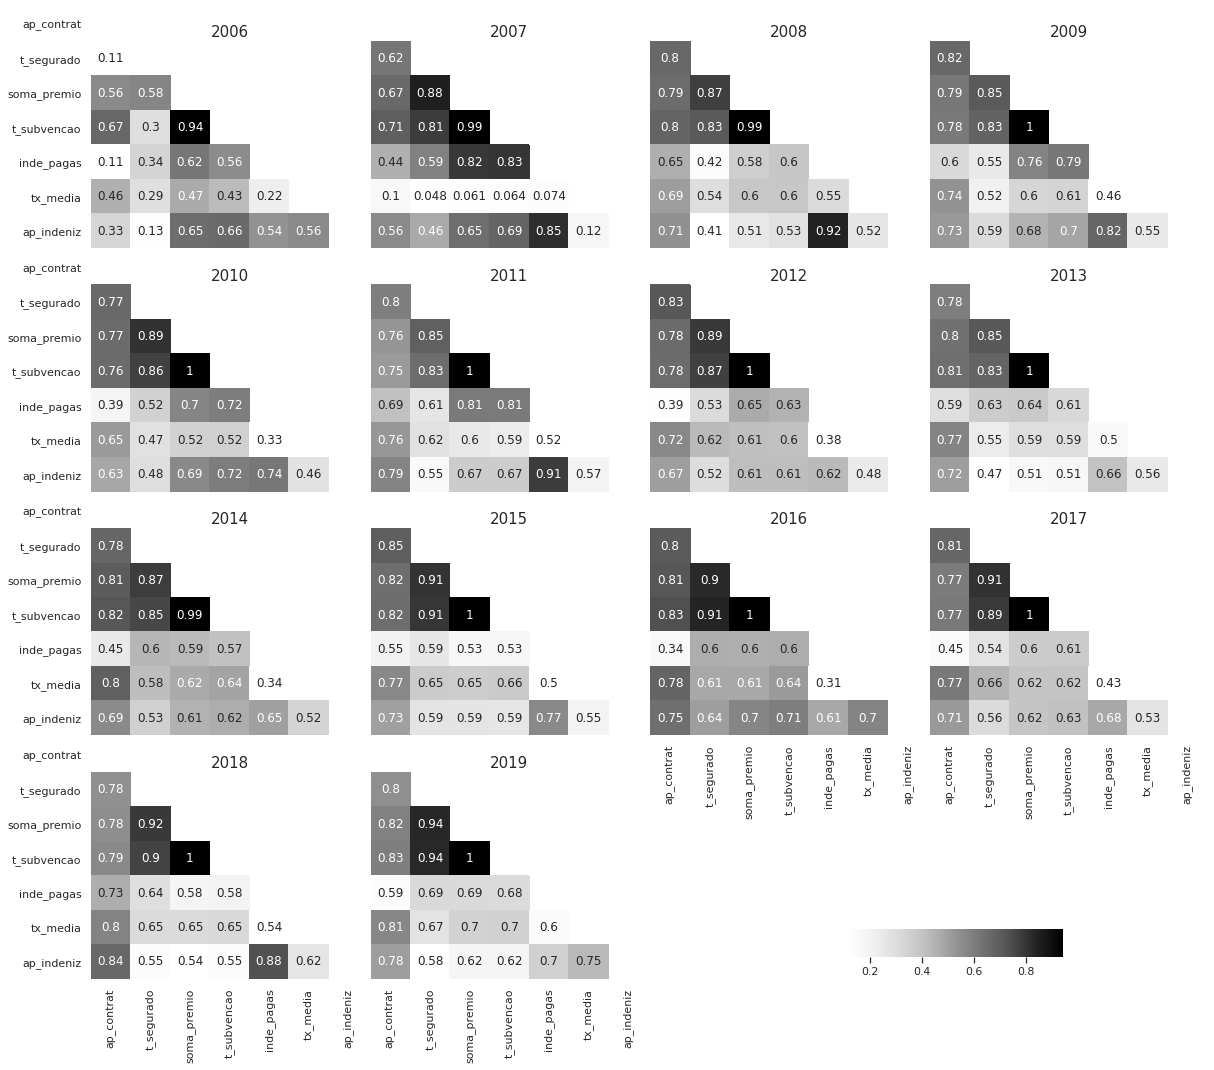
\includegraphics[width=0.9\textwidth]{figuras/corr_anos_bw.png}
	\parbox{\dimexpr\linewidth-2cm}{\raggedright
    \strut \textsuperscript{Fonte: Elaboração própria}\strut}
    \label{corr_anos}
\end{figure}

\subsection{ANÁLISE DE COMPONENTES PRINCIPAIS} 

\begin{small}
\begin{table}[H]
\caption{Proporção da variância explicada acumulada pelos componentes principais. Brasil $2006$ -- $2019$} \label{tab_var_ratio}
%\caption{I de Moran para as variáveis de seguro rural no Brasil por municípios entre 2006 e 2019} 
\footnotesize
\vspace{0.05cm}
\label{moran_table}
\begin{tabularx}{\textwidth}{lXXXXXXX}
    \hline \\[-1.9ex]	 
    Anos & CP1 & CP2 & CP3 & CP4 & CP5 & CP6 & CP7 \\
    \hline \\[-1.9ex]	 
    2006 &  0.5530 &  0.1542 &  0.1233 &  0.1029 &  0.0437 &  0.0226 &  0.0003 \\
    2007 &  0.6514 &  0.1433 &  0.1043 &  0.0703 &  0.0232 &  0.0073 &  0.0002 \\
    2008 &  0.7154 &  0.1497 &  0.0721 &  0.0377 &  0.0181 &  0.0064 &  0.0005 \\
    2009 &  0.7491 &  0.0974 &  0.0815 &  0.0443 &  0.0144 &  0.0129 &  0.0003 \\
    2010 &  0.7076 &  0.1222 &  0.0917 &  0.0475 &  0.0188 &  0.0119 &  0.0003 \\
    2011 &  0.7643 &  0.0945 &  0.0856 &  0.0363 &  0.0150 &  0.0041 &  0.0003 \\
    2012 &  0.7141 &  0.1114 &  0.0815 &  0.0582 &  0.0228 &  0.0117 &  0.0003 \\
    2013 &  0.7180 &  0.1120 &  0.0803 &  0.0474 &  0.0302 &  0.0118 &  0.0004 \\
    2014 &  0.7186 &  0.1126 &  0.0839 &  0.0452 &  0.0269 &  0.0122 &  0.0006 \\
    2015 &  0.7433 &  0.1188 &  0.0689 &  0.0398 &  0.0203 &  0.0086 &  0.0002 \\
    2016 &  0.7414 &  0.1171 &  0.0785 &  0.0332 &  0.0189 &  0.0106 &  0.0003 \\
    2017 &  0.7286 &  0.1070 &  0.0827 &  0.0483 &  0.0211 &  0.0123 &  0.0001 \\
    2018 &  0.7564 &  0.1313 &  0.0674 &  0.0243 &  0.0154 &  0.0051 &  0.0001 \\
    2019 &  0.7797 &  0.0975 &  0.0676 &  0.0314 &  0.0141 &  0.0097 &  0.0001 \\
	\hline 
\end{tabularx}
%\vspace{0.5cm}
\footnotesize{Fonte: Elaboração própria.  }\\

\end{table}
\end{small}


\begin{figure}[H]
	\centering
	\caption{Variância explicada acumulada pelos componentes principais. Brasil $2006$ -- $2019$}
	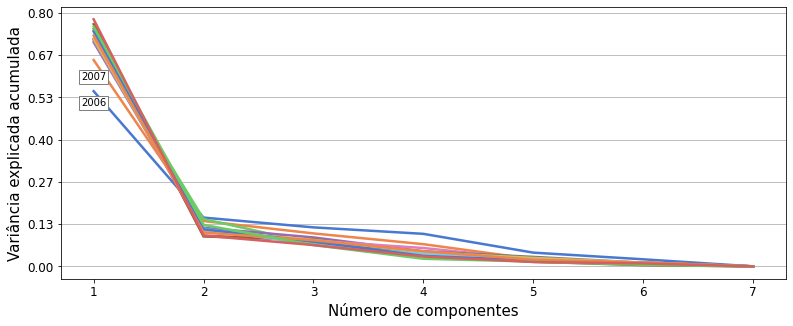
\includegraphics[width=0.8\textwidth]{figuras/var_radio.png}\\
	\small \textsuperscript {Fonte: Elaboração própria}
    \label{var_ratio}
\end{figure}

Devido à estrutura de correlação entre as variáveis de seguro rural foi possível utilizar os escores do primeiro componente principal como uma variável representativa das demais variáveis originais. A correlação dos escores do primeiro componente principal foram, em todos os anos, positivamente correlacionados com todas as variáveis originais. Além disso, em todos os anos analisados, a variância explicada acumulada pelo primeiro componente foi superior à $55,3\%$. 

%\begin{figure}[H]
%	\centering
%	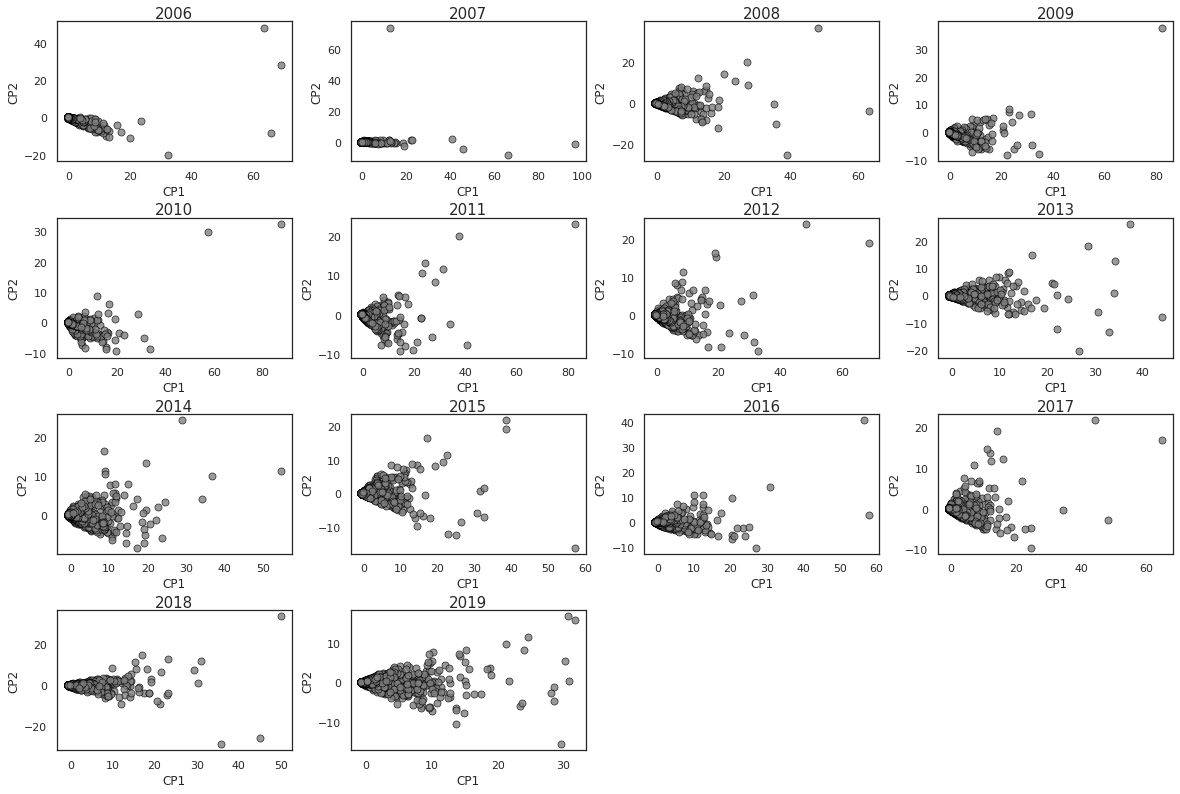
\includegraphics[width=1\textwidth]{figuras/cp1_cp2.png}
%	\caption{Diagrama de dispersão entre os dois primeiros componentes. Brasil $2006$ -- $2019$}
%	\small \textsuperscript {Fonte: Elaboração própria}
%    \label{corr_anos}
%\end{figure}

\begin{figure}[H]
	\centering
	\caption{Diagrama de dispersão entre os dois primeiros componentes. Brasil $2006$ -- $2019$}
	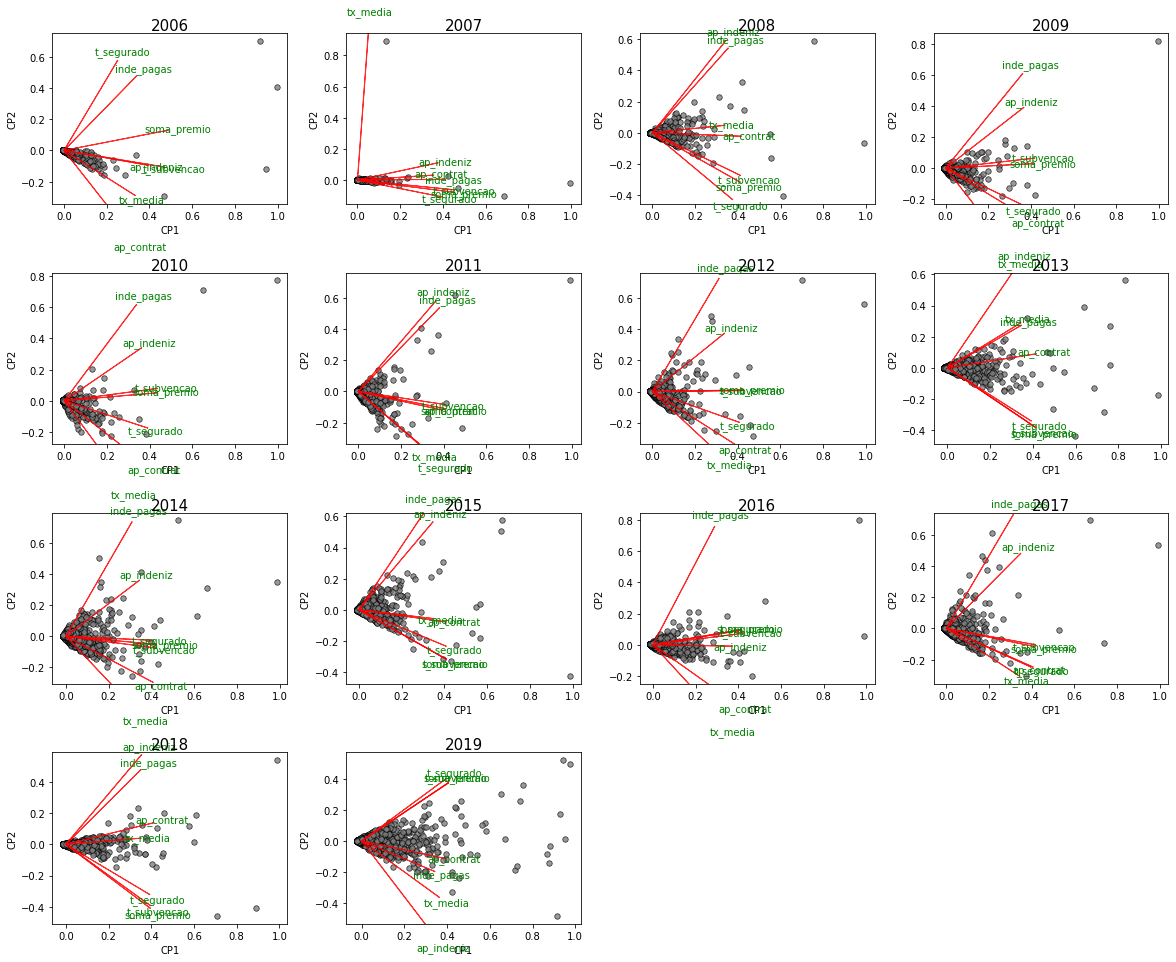
\includegraphics[width=1\textwidth]{figuras/acp_biplot.png}
	\small \textsuperscript {Fonte: Elaboração própria}
    \label{acp_biplot}
\end{figure}

\begin{figure}[H]
	\centering
	\caption{Correlação entre as variáveis de seguro Rural. Brasil $2006$ -- $2019$.}
	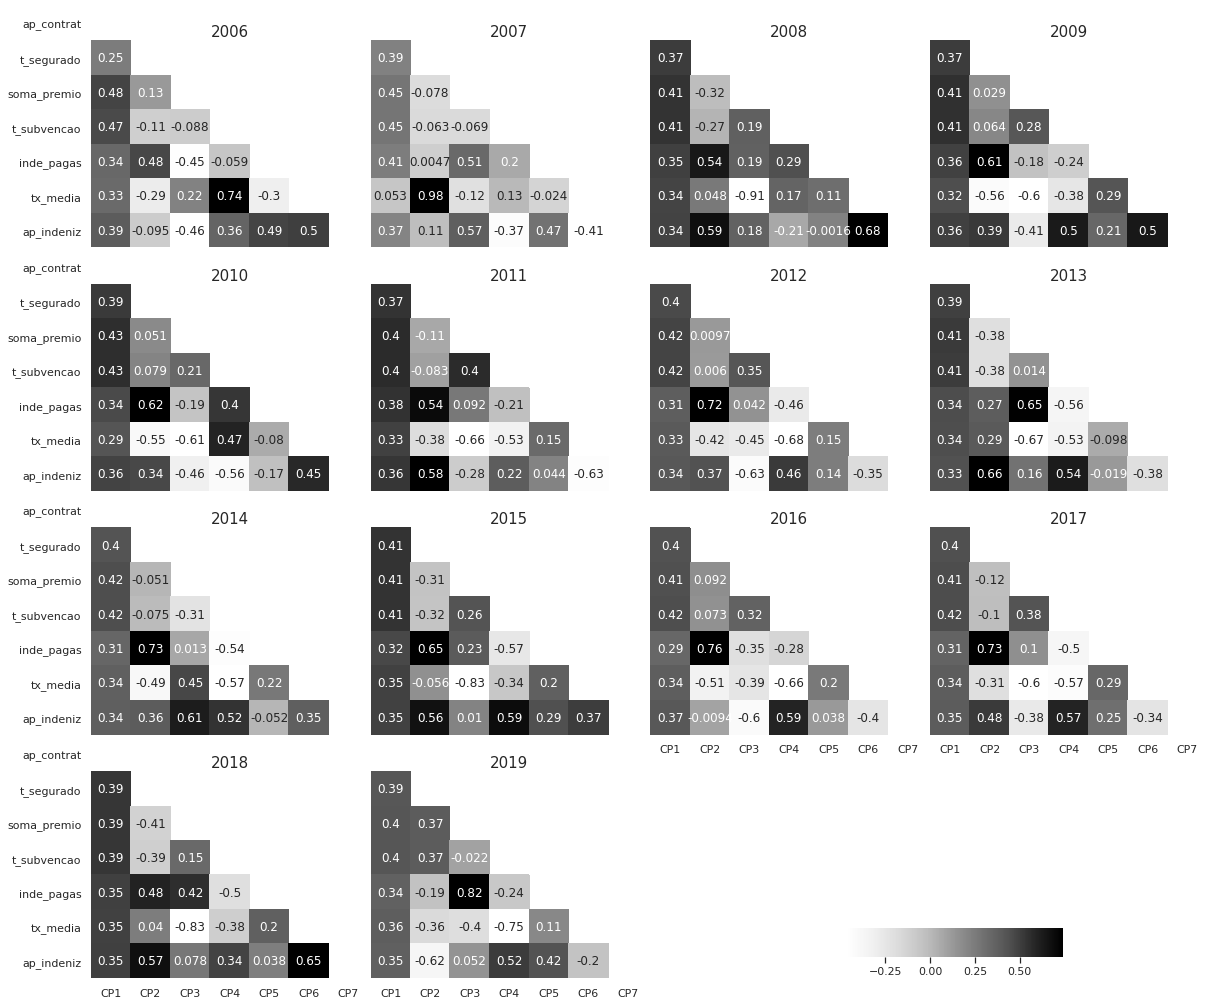
\includegraphics[width=0.9\textwidth]{figuras/corr_pca_var.png}
	\small \textsuperscript {Fonte: Elaboração própria.}
    \label{corr_pca_var}
\end{figure}

\subsection{ANÁLISE EXPLORATÓRIA DE DADOS ESPACIAIS}


\begin{figure}[H]
	\centering
	\caption{Distribuição espacial do primeiro componente principal. Brasil $2006$ -- $2019$.}
	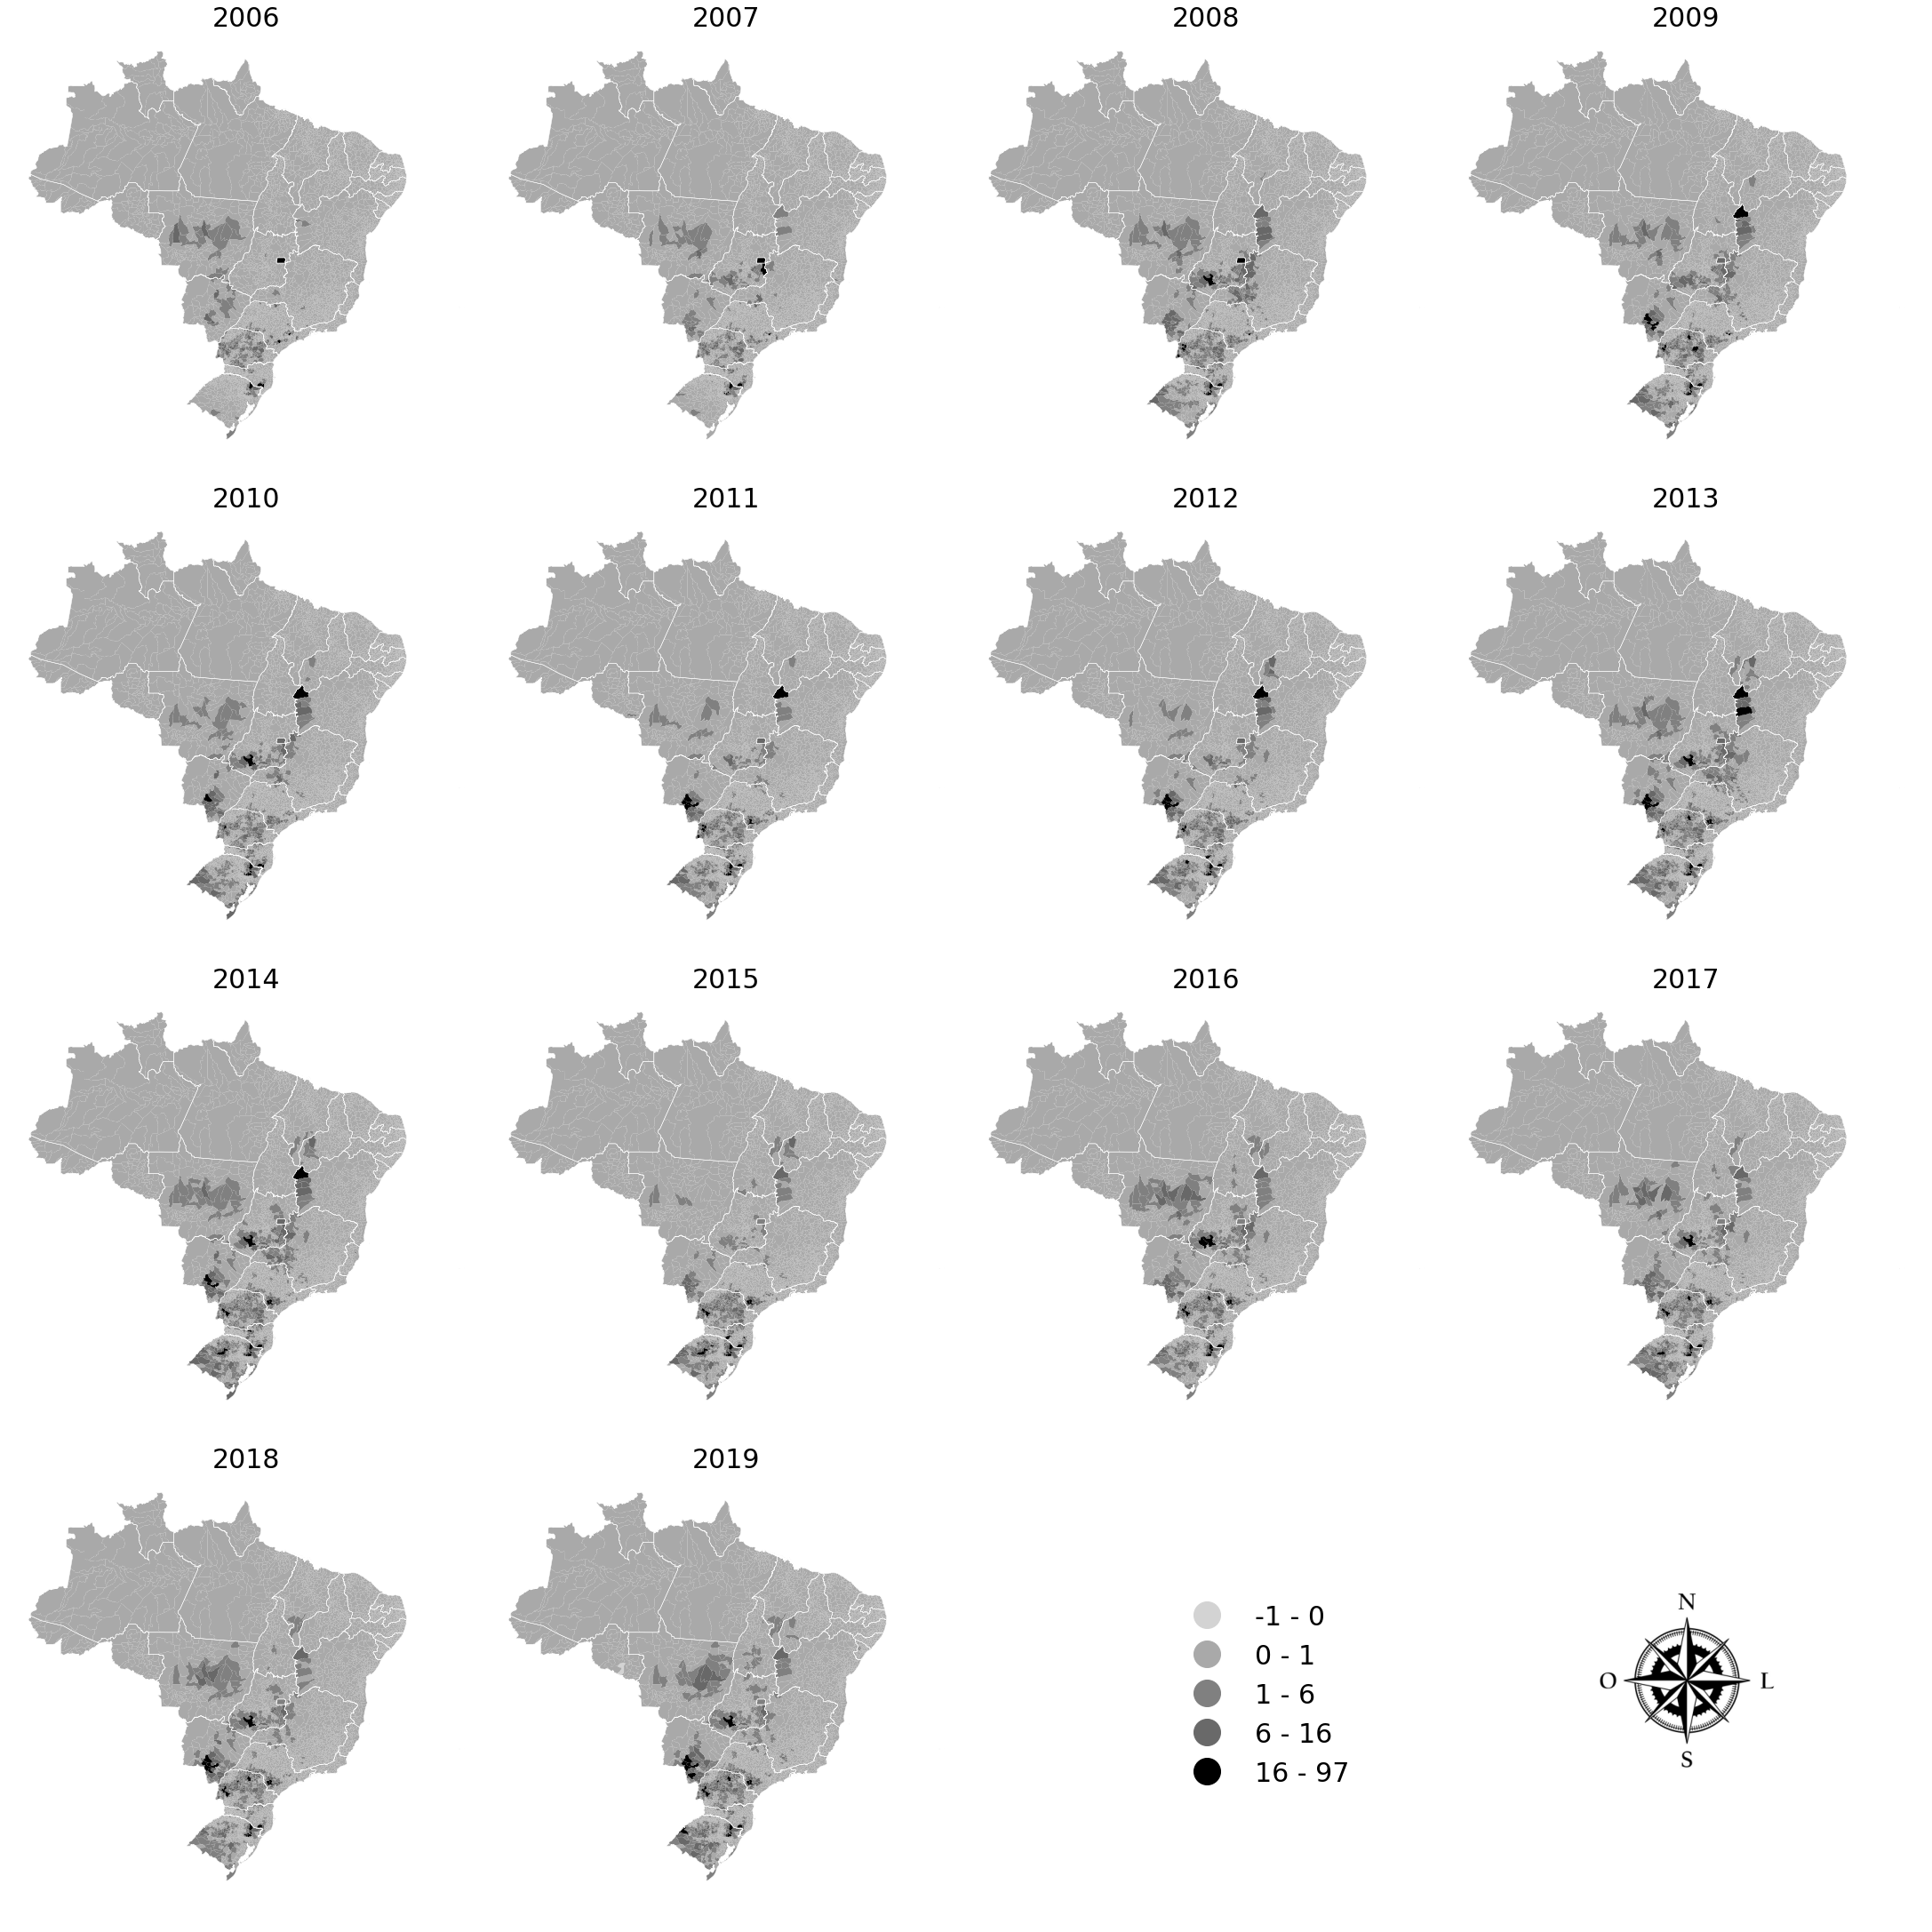
\includegraphics[width=0.9\textwidth]{figuras/map_CP1.png}\\
	\small \textsuperscript {Fonte: Elaboração própria.}
    \label{map_cp1}
\end{figure}

\begin{figure}[H]
	\centering
	\caption{Autocorrelação espacial (\textit{I} de Moran) do primeiro componente principal. Brasil $2006$ -- $2019$}
	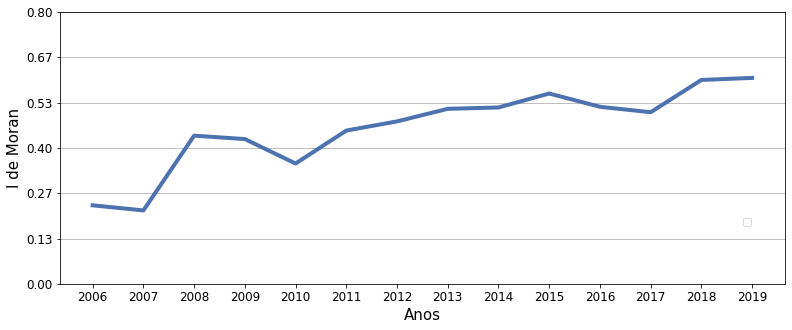
\includegraphics[width=0.8\textwidth]{figuras/i_de_moran_cp1.png}\\
	\small \textsuperscript {Fonte: Elaboração própria.}
    \label{i_moran_cp1}
\end{figure}


\begin{figure}[H]
	\centering
	\caption{Mapas \textit{LISA} para o primeiro componente principal.  Brasil $2006$ -- $2019$.}
	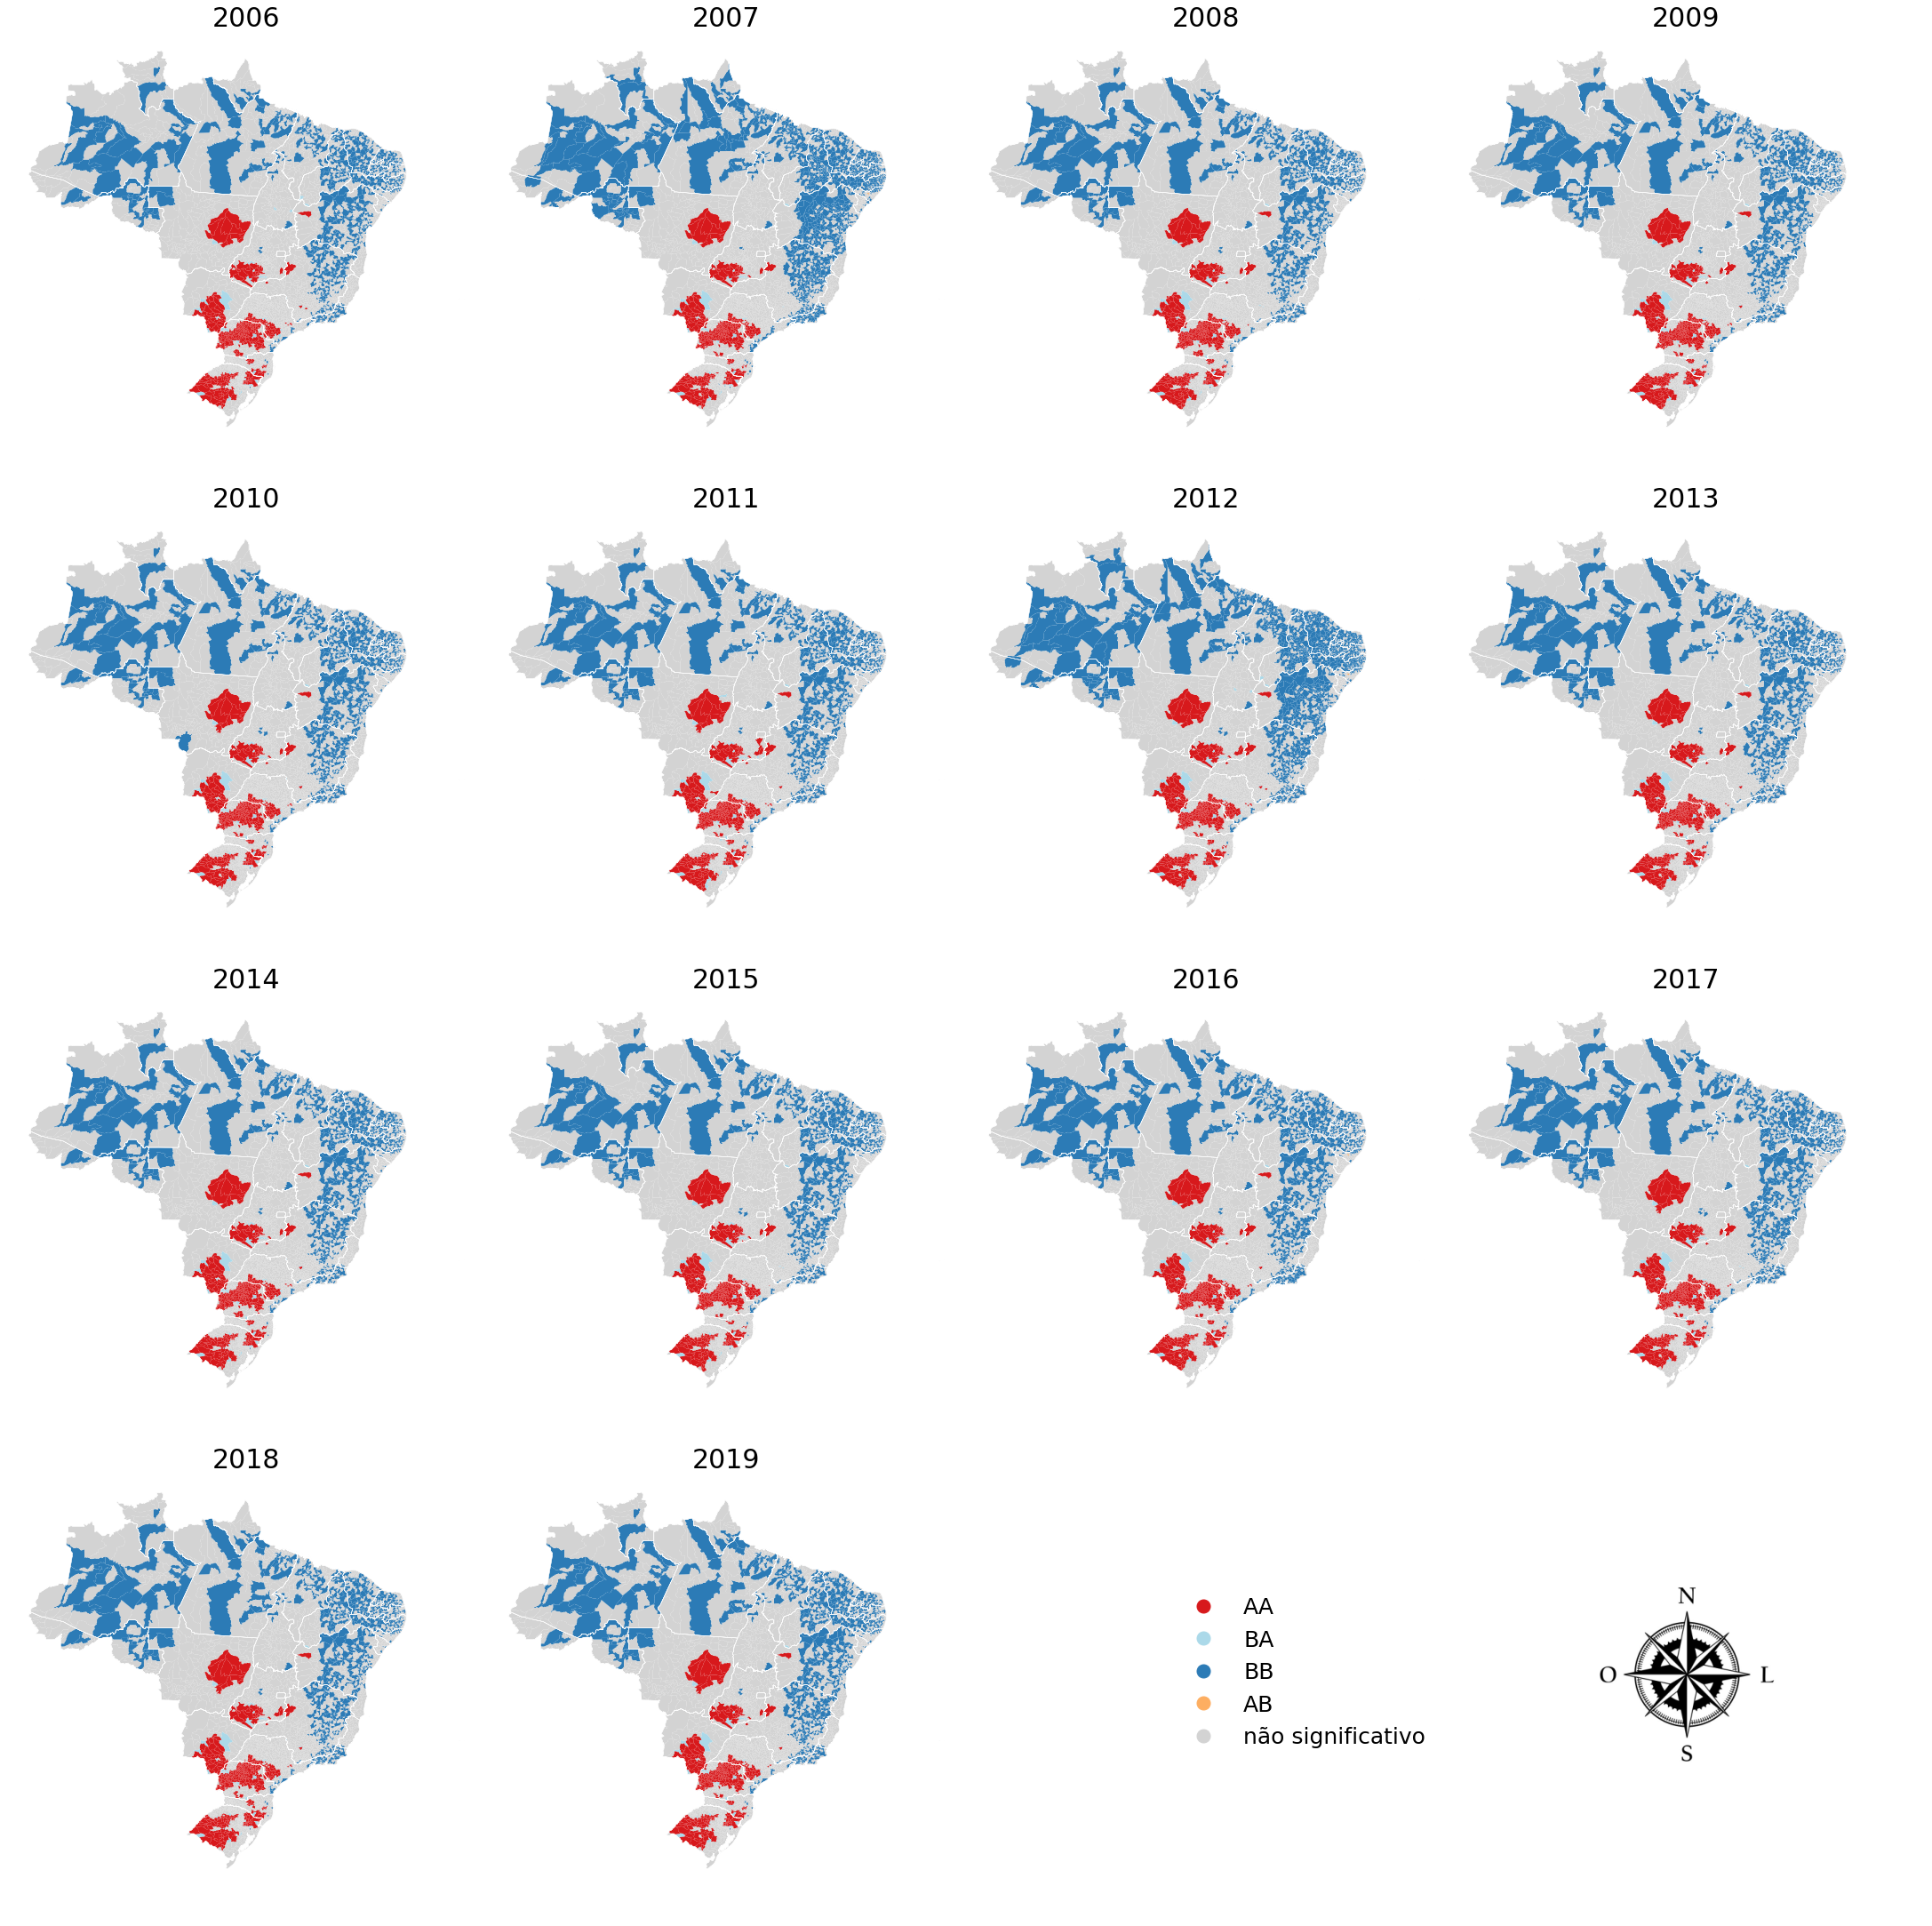
\includegraphics[width=0.9\textwidth]{figuras/map_lisa_cp1.png}\\
	\small \textsuperscript {Fonte: Elaboração própria.}
    \label{map_lisa_cp1}
\end{figure}

\section{CONSIDERAÇÕES FINAIS}\label{sc-conclusion}

\newpage
\addcontentsline{toc}{section}{\hspace*{\distnumber}REFERÊNCIAS}
\begin{center}
\section*{REFERÊNCIAS} 
\end{center}

    
% Use isso descomentado durante edição.
% Quando concluir a Tese, comente iss e use
% o código do bloco abaixo.
%\begin{singlespace}
%\renewcommand\refname{}
%\begin{flushleft}
%\bibliography{../tese/bibtese2}
%\end{flushleft}
%\end{singlespace}

%% Em cap2nlme-corrigido.bbl foi feita correção manual de
%% algumas referências como por exemplo as citações
%% de Dissertação e Tese.
%% Então deixa-se de usar o arquivo cap2nlme.bbl gerado
%% automaticamente pelo abntcite, mas isso é só ao final.
\begin{singlespace}
\begin{flushleft}
\renewcommand\refname{}
\vspace*{-1.5cm}
%==========================================================================================

\documentclass[10pt]{article}

%==========================================================================================

\usepackage[utf8]{inputenc}
\usepackage[brazil]{babel}
\usepackage[T1]{fontenc}
\usepackage{amsmath}
\usepackage{amsfonts}
\usepackage{mathrsfs}
\usepackage{amssymb}
\usepackage{graphicx}
\usepackage{geometry, calc, color, setspace}
\usepackage{indentfirst}
\usepackage{wrapfig}
\usepackage{boxedminipage}
\usepackage{enumerate}
\usepackage{float}
\usepackage{paralist}
\usepackage{comment}
\usepackage{icomma}
\usepackage{rotating}
\usepackage{multirow}
\usepackage[position=bottom]{subfig}
\usepackage{array}
\usepackage{tabularx}
\usepackage{float}
\usepackage{array}

\newcolumntype{L}[1]{>{\raggedright\let\newline\\\arraybackslash\hspace{0pt}}m{#1}}
\newcolumntype{C}[1]{>{\centering\let\newline\\\arraybackslash\hspace{0pt}}m{#1}}
%\newcolumntype{R}[1]{>{\raggedleft\let\newline\\\arraybackslash\hspace{0pt}}m{#1}}
\newcolumntype{R}{>{\raggedleft\let\newline\\\arraybackslash\hspace{0pt}}X}

\usepackage[alf,bibjustif]{abntex2cite}
%\usepackage{abntcite}

% Para o alinhamento dos títulos das figuras
\usepackage{caption}
%\captionsetup[figure]{format=hang,labelsep=endash,font=small,justification=RaggedRight,singlelinecheck=off, margin=1cm}
\captionsetup[subfigure]{textfont=small,singlelinecheck=off,justification=raggedright}


%%  Inserindo os códigos Python ==================================
\usepackage{listings}

%\definecolor{light_gray}{rgb}{0.97,0.97,0.97}
%\definecolor{mymauve}{rgb}{0.58,0,0.82}
%\definecolor{mygreen}{rgb}{0,0.6,0}

\lstset{
  language = Python,
  inputencoding = utf8,
  backgroundcolor = \color{white},
  columns=fullflexible,
  basicstyle=\ttfamily,
  breaklines=true,
  postbreak=\raisebox{0ex}[0ex][0ex]{\color{black}$\hookrightarrow$\space},
  keywordstyle=\color{black},      % keyword style
  stringstyle=\color{black},
  commentstyle=\color{black}
}

\newcommand{\HRule}{\noindent\rule{\linewidth}{0.2mm}}

\usepackage{mathpazo}                         % tem suporte matemático
\usepackage[scaled=0.85]{beramono}            % usa esta nos verbatins [scaled=0.9]

\renewcommand\UrlFont{\color{black}\rmfamily} 

\def\distnumber{2.3em}

%==========================================================================================

\author{Walef Machado de Mendonça\footnote{Mestrando em Estatística Aplicada e Biometria na Universidade Federal de Alfenas}\\
Patrícia de Siqueira Ramos\footnote{Professora da Universidade Federal de Alfenas, campus Varginha}}

%==========================================================================================


\title{Análise de autocorrelação espacial de dados multivariados de seguro rural}
\date{}

\begin{document}

\maketitle

\begin{abstract}
\noindent O ambiente no qual se desenvolvem as atividades agropecuárias apresenta elevado risco e grande incerteza. Diversos fatores relacionados ao setor agropecuário podem gerar oscilações na renda dos produtores. Estas oscilações devem ser enfrentadas por meio de políticas de apoio à gestão de riscos como, por exemplo, a contratação de seguro rural. Esta modalidade de seguro possibilita a recuperação da capacidade financeira do produtor na ocorrência de eventos adversos que causem prejuízo econômico. Considerando a relevância do seguro rural no setor agropecuário, este trabalho tem como objetivo avaliar a distribuição espacial das variáveis desse seguro nos municípios brasileiros no período de 2006 a 2019. Para alcançar tal objetivo, foi utilizada a Análise de Componentes Principais, com o objetivo de reduzir a dimensionalidade dos dados e a Análise Exploratória de Dados Espaciais para investigar a presença de padrões de distribuição espacial do seguro rural. Os dados utilizados são provenientes dos censos do seguro rural, compilados pelo Ministério da Agricultura, Pecuária e Abastecimento. Com a utilização de escores dos CPs, verificou-se que as maiores concentrações de apólices de seguro rural estão situadas nas regiões Sul e Centro-Oeste e há uma tendência de aumento na dependência espacial do seguro rural ao longo do período analisado. \\
\newline
\noindent {\textbf{Palavras-chave}}: Seguro rural. Política agrícola. Estatística espacial. Autocorrelação espacial. I de Moran.
\end{abstract}


\section{INTRODUÇÃO}

As atividades agropecuárias têm grande relevância na economia brasileira. Segundo um estudo realizado pelo Centro de Estudos Avançados em Economia Aplicada (CEPEA), da Esalq/USP, a parcela da participação do agronegócio no PIB brasileiro foi de $20,5\%$ em $2019$, e em $2020$, este percentual chegou à $26,6\%$ \cite{cepea21_2}. De acordo com o último Censo Agropecuário, entre $2006$ e $2017$, houve um acréscimo de cerca de $5,8\%$ na área total dos estabelecimentos agropecuários e, tanto a área total quanto a produção agrícola e pecuária apresentaram um considerável crescimento \cite{ibge19_2}.

No entanto, o ambiente no qual se desenvolvem as atividades agropecuárias apresenta elevado risco e significativa incerteza. Essa insegurança se deve, principalmente, às instabilidades climáticas e ameaças sanitárias, que podem afetar a produção, ou à razões de mercado, como variações das taxas de câmbio e juros, ou a condições ligadas ao ambiente de negócios, tais como alterações em marcos regulatórios e em políticas públicas. Todas essas variáveis, relacionadas aos mercados agropecuários, geram variações na renda do setor, que são comumente enfrentadas por meio de políticas de apoio à gestão de riscos \cite{brasil18_2}.

O gerenciamento de riscos agropecuários pode ocorrer de diversas maneiras. No entanto, a contratação de seguro rural é uma das formas mais usuais. Essa modalidade de seguro atua no sentido de amenizar as perdas e possibilitar a recuperação da capacidade financeira do produtor na ocorrência de sinistros. O seguro rural propicia um ambiente mais favorável ao desenvolvimento das atividades agropecuárias, pois proporciona a garantia do fluxo de renda, favorece um aumento da área plantada e facilita a obtenção de financiamento. Além disso, se mostra um instrumento que possibilita o compartilhamento do risco da agropecuária com outros agentes e setores econômicos \cite{brasil19_2}.

%É importante destacar que o mercado de seguro rural não se consolida sem a participação do Estado. Destacam-se problemas como os elevados investimentos e custos administrativos, a possibilidade de riscos catastróficos, a forte influência do risco moral e da seleção adversa na formação das carteiras, como fatores que limitam a eficiência da iniciativa privada na oferta de produtos. Nesse sentido, o poder público é demandado a interferir no mercado, seja atuando diretamente como seguradora, seja criando programas que estimulem a oferta e a demanda por produtos de seguro (BRASIL, 2019a). 

% Esses dois estão ok...

Considerando a relevância do seguro rural no setor agropecuário, este estudo tem como objetivo analisar a distribuição espacial de dados multivariados do seguro rural nos municípios brasileiros entre os anos de $2006$ e $2019$. Além disso, busca-se investigar a presença de padrões de distribuição espacial nos dados, mais especificamente, se há presença de dependência ou heterogeneidade espacial. Por fim, este trabalho pretende fornecer informações que possam contribuir para o debate em torno do aperfeiçoamento do sistema de seguro rural no Brasil. Para alcançar tais objetivos, o trabalho faz uso da Análise de Componentes Principais (ACP) para reduzir a dimensionalidade dos dados e da Análise Exploratória de Dados Espaciais (AEDE), para investigar a presença de padrões de distribuição espacial. São utilizados dados oriundos dos Censos do Seguro Rural, compilados pelo Ministério da Agricultura, Pecuária e Abastecimento \cite{brasil21}.

O trabalho estrutura-se da seguinte forma: na seção $2$ é apresentado uma revisão de literatura a respeito do seguro rural no Brasil, assim como a Análise de Componentes Principais e a Análise Exploratória de Dados Espaciais. A seção $3$ descreve a metodologia utilizada neste estudo, a fonte dos dados e os recursos computacionais. A seção $4$ discute os resultados obtidos. Por fim, a seção $5$ traz as considerações finais. 


%Ao longo dos últimos anos, o agronegócio tem sido o único setor da economia brasileira que vem mantendo crescimento. Esse resultado é fruto do aumento na área plantada com as principais culturas, e, principalmente, dos investimentos em máquinas, equipamentos e tecnologias e, em consequência, do aumento da produtividade no campo.

%Apesar desses resultados positivos, mesmo em anos de safras recordes, eventos climáticos de abrangência regional têm afetado os produtores, causando perdas significativas em suas lavouras e na sua rentabilidade

%\section{REFERENCIAL TEÓRICO}\label{referencial}

\section{MATERIAL E MÉTODOS}\label{methods}

Nesse trabalho, foi utilizada a análise exploratória de dados espaciais com o objetivo de avaliar a distribuição espacial do seguro rural nos municípios brasileiros no período de $2006$ a $2019$. Inicialmente, foi realizada uma análise exploratória dos dados de forma a auxiliar a análise de componentes principais e análise exploratória espacial. O resumo estatístico das variáveis estudadas foi obtido e, de modo a identificar os pares de variáveis mais associadas entre si, foram calculadas as matrizes de correlações de Pearson entre as variáveis, para cada um dos anos entre $2006$ e $2019$. A matriz de correlações linear tem a forma apresentada na definição (\ref{def_matriz_corr_2}).

Após a análise exploratória, foi empregada a análise de componentes principais (ACP) com o objetivo de reduzir a dimensionalidade dos dados. O método foi aplicado com a intenção de reduzir o conjunto das variáveis originais correlacionadas entre si a um novo conjunto de variáveis, os componentes principais (CPs), não correlacionadas. Os escores, valores numéricos dos componentes, do primeiro componente principal (CP1) foram utilizados para a análise exploratória de dados espaciais (AEDE). 

Para a realização da AEDE, é necessária a utilização da matriz de pesos espaciais apresentada na subseção \ref{W_matrix_2}. Para a construção dessa matriz de pesos espaciais, foram desconsiderados os municípios de Fernando de Noronha (PE) e Ilhabela (SP). Esses municípios foram retirados da análise pois, além de se constituírem de ilhas, não possuem nenhuma apólice de seguro rural contratada durante os anos analisados. 

% Dados
Foram utilizados dados anuais referentes a apólices de seguro rural dos municípios brasileiros a partir do ano de $2006$ até o ano de $2019$ (último ano disponível até então). As variáveis utilizadas na análise são apresentadas na Tabela \ref{tab_variaveis}. Para todas as variáveis, foi utilizado o nível de agregação municipal. Nos casos em que as informações disponíveis eram referentes a outras localidades, como distritos, fazendas e vilarejos, tais informações foram atribuídas aos municípios correspondentes. 

\begin{small}
\begin{table}[!htp]
\caption{Descrição das variáveis utilizadas.}\label{tab_variaveis}
 \begin{center}
\begin{tabular}{ll}
\hline 
Sigla & Variável  \tabularnewline
\hline 
ap\_contrat    & Total de apólices contratadas                         \\
t\_segurado    & Soma da importância segurada (R\$ milhão)             \\
soma\_premio   & Soma dos prêmios (R\$ milhão)                         \\
t\_subvencao   & Total de subvenção (R\$ milhão)                       \\
inde\_pagas    & Soma das indenizações pagas (R\$ milhão)              \\
tx\_media      & Taxa média aplicada às apólices                       \\
ap\_indeniz    & Número de apólices indenizadas                        \\ 
%\tabularnewline
\hline 
\vspace{0.1cm}
\footnotesize{Fonte: Elaboração própria}
%\end{tabular}
\end{tabular}
\end{center}
\end{table}
\end{small}
	
% Fonte dos Dados 
Os dados sobre seguro rural estão disponíveis no endereço eletrônico do Ministério da Agricultura, Pecuária e Abastecimento (MAPA). Os dados que contém atributos geográficos, como a posição e o formato, do território brasileiro estão disponíveis no endereço eletrônico do Instituto Brasileiro de Geografia e Estatística (IBGE, 2020).
	
%Padronização
Como as variáveis estão em diferentes escalas e, com isto, possuem diferentes variâncias, foi realizada a padronização das variáveis para que tais fatores não interferissem na análise. Tal padronização foi efetuada subtraindo-se de cada observação a média de sua respectiva variável e dividindo-se posteriormente pelo desvio padrão da variável.

% Linguagem de programação 
Esse estudo foi realizado com a linguagem de programação \textit{Python} \cite{python17_2}, utilizando-se a interface \textit{Jupyter} \cite{jupyter17_2}, \cite{perez07_2} \cite{kluyver19_2}.
Além disso, as seguintes bibliotecas foram utilizadas: 
\textit{Pandas} \cite{mckinney10_2}, para a manipulação de dados,
\textit{NumPy} \cite{walt11_2}, que possibilita computação numérica com \textit{Python},
\textit{Matplotlib} \cite{hunter07_2} e \textit{Seaborn} \cite{waskom14_2}, que são bibliotecas para a criação de gráficos,
\textit{jenkspy} para a utilização do algoritmo Fisher Jenks \cite{jenks77_2}. 
A análise de componentes principais foi realizada através da biblioteca \textit{sklearn} e as bibliotecas \textit{Geopandas} \cite{jordahl14_2} e \textit{PySAL} \cite{rey07_2} possibilitaram a análise espacial.

% Fisher-Jenks. Tal método, segundo \citeonline{rey2013}, é frequentemente recomendado por cartógrafos, sendo apresentado por \citeonline{jenks1977} e originalmente proposto por \citeonline{fisher1958}, a abordagem baseia-se no particionamento ideal de dados univariados. 

%@article{rey2013,
%  title={Parallel optimal choropleth map classification in PySAL},
%  author={Rey, Sergio and Anselin, Luc and Pahle, Robert and Kang, Xing and Stephens, Philip},
%  journal={International Journal of Geographical Information Science},
%  volume={27},
%  number={5},
%  pages={1023--1039},
%  year={2013},
%  publisher={Taylor \& Francis}
%}

%@article{fisher1958,
%  title={On grouping for maximum homogeneity},
%  author={Fisher, Walter},
%  journal={Journal of the American statistical Association},
%  volume={53},
%  number={284},
%  pages={789--798},
%  year={1958},
%  publisher={Taylor \& Francis}
%}

%@article{jenks1977,
%  title={Optimal data classification for choropleth maps},
%  author={Jenks, George},
%  journal={Department of Geography, University of Kansas Occasional Paper},
%  year={1977}
%}


\section{RESULTADOS E DISCUSSÃO}\label{sc-results}

\subsection{CORRELAÇÃO ENTRE AS VARIÁVEIS} 

A Figura \ref{corr_anos} apresenta os valores das correlações de Pearson entre cada um dos pares de variáveis de seguro rural utilizadas. Quanto mais escura a cor do retângulo mais próximo de $1$ é o valor do coeficiente de correlação e, portanto, maior o grau de associação entre as variáveis. Por outro lado, quanto mais clara a cor do retângulo, mais próximo de $0$ é o valor do coeficiente de correlação e, portanto, menor o grau de associação entre as variáveis\footnote{Esta representação com escala em cinza foi escolhida por não haver, nos dados analisados, a presença de correlação negativa.}.

\begin{figure}[H]
	\centering
	\caption{Correlação entre as variáveis de seguro Rural. Brasil $2006$ -- $2019$}
	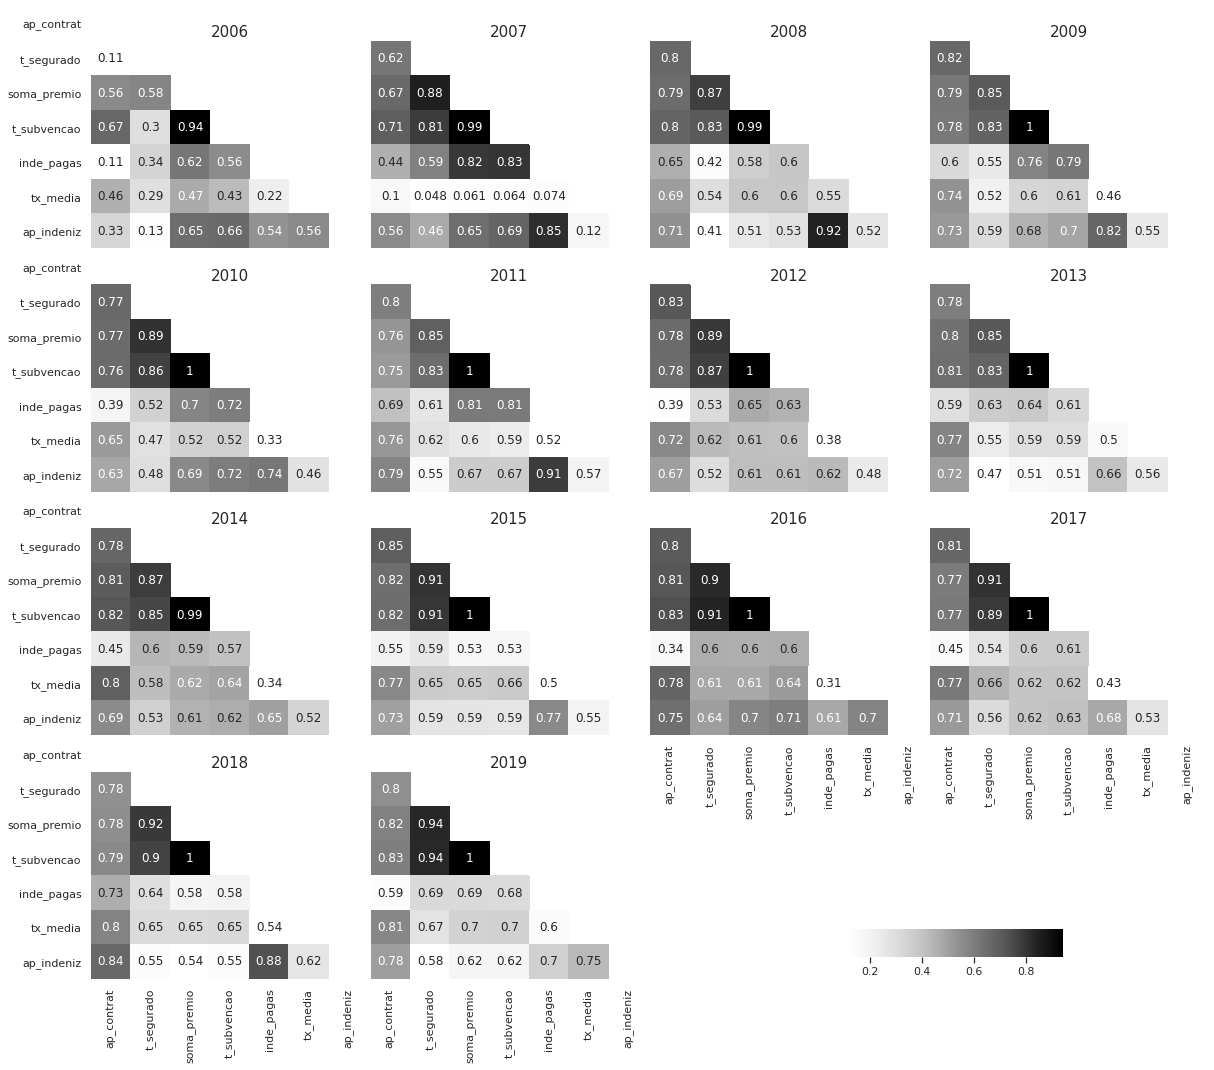
\includegraphics[width=0.9\textwidth]{figuras/corr_anos_bw.png}
	\parbox{\dimexpr\linewidth-2cm}{\raggedright
    \strut \textsuperscript{Fonte: Elaboração própria}\strut}
    \label{corr_anos}
\end{figure}

\subsection{ANÁLISE DE COMPONENTES PRINCIPAIS} 

\begin{small}
\begin{table}[H]
\caption{Proporção da variância explicada acumulada pelos componentes principais. Brasil $2006$ -- $2019$} \label{tab_var_ratio}
%\caption{I de Moran para as variáveis de seguro rural no Brasil por municípios entre 2006 e 2019} 
\footnotesize
\vspace{0.05cm}
\label{moran_table}
\begin{tabularx}{\textwidth}{lXXXXXXX}
    \hline \\[-1.9ex]	 
    Anos & CP1 & CP2 & CP3 & CP4 & CP5 & CP6 & CP7 \\
    \hline \\[-1.9ex]	 
    2006 &  0.5530 &  0.1542 &  0.1233 &  0.1029 &  0.0437 &  0.0226 &  0.0003 \\
    2007 &  0.6514 &  0.1433 &  0.1043 &  0.0703 &  0.0232 &  0.0073 &  0.0002 \\
    2008 &  0.7154 &  0.1497 &  0.0721 &  0.0377 &  0.0181 &  0.0064 &  0.0005 \\
    2009 &  0.7491 &  0.0974 &  0.0815 &  0.0443 &  0.0144 &  0.0129 &  0.0003 \\
    2010 &  0.7076 &  0.1222 &  0.0917 &  0.0475 &  0.0188 &  0.0119 &  0.0003 \\
    2011 &  0.7643 &  0.0945 &  0.0856 &  0.0363 &  0.0150 &  0.0041 &  0.0003 \\
    2012 &  0.7141 &  0.1114 &  0.0815 &  0.0582 &  0.0228 &  0.0117 &  0.0003 \\
    2013 &  0.7180 &  0.1120 &  0.0803 &  0.0474 &  0.0302 &  0.0118 &  0.0004 \\
    2014 &  0.7186 &  0.1126 &  0.0839 &  0.0452 &  0.0269 &  0.0122 &  0.0006 \\
    2015 &  0.7433 &  0.1188 &  0.0689 &  0.0398 &  0.0203 &  0.0086 &  0.0002 \\
    2016 &  0.7414 &  0.1171 &  0.0785 &  0.0332 &  0.0189 &  0.0106 &  0.0003 \\
    2017 &  0.7286 &  0.1070 &  0.0827 &  0.0483 &  0.0211 &  0.0123 &  0.0001 \\
    2018 &  0.7564 &  0.1313 &  0.0674 &  0.0243 &  0.0154 &  0.0051 &  0.0001 \\
    2019 &  0.7797 &  0.0975 &  0.0676 &  0.0314 &  0.0141 &  0.0097 &  0.0001 \\
	\hline 
\end{tabularx}
%\vspace{0.5cm}
\footnotesize{Fonte: Elaboração própria.  }\\

\end{table}
\end{small}


\begin{figure}[H]
	\centering
	\caption{Variância explicada acumulada pelos componentes principais. Brasil $2006$ -- $2019$}
	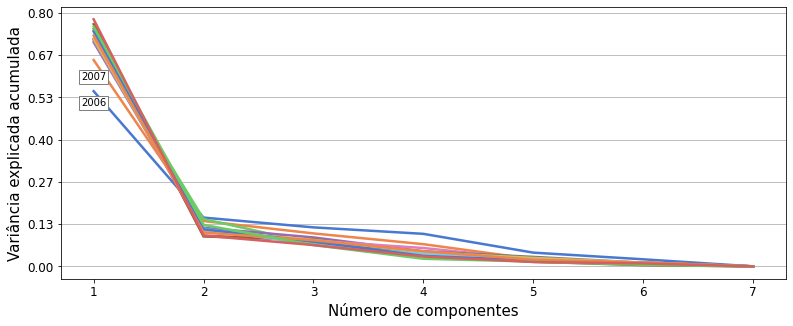
\includegraphics[width=0.8\textwidth]{figuras/var_radio.png}\\
	\small \textsuperscript {Fonte: Elaboração própria}
    \label{var_ratio}
\end{figure}

Devido à estrutura de correlação entre as variáveis de seguro rural foi possível utilizar os escores do primeiro componente principal como uma variável representativa das demais variáveis originais. A correlação dos escores do primeiro componente principal foram, em todos os anos, positivamente correlacionados com todas as variáveis originais. Além disso, em todos os anos analisados, a variância explicada acumulada pelo primeiro componente foi superior à $55,3\%$. 

%\begin{figure}[H]
%	\centering
%	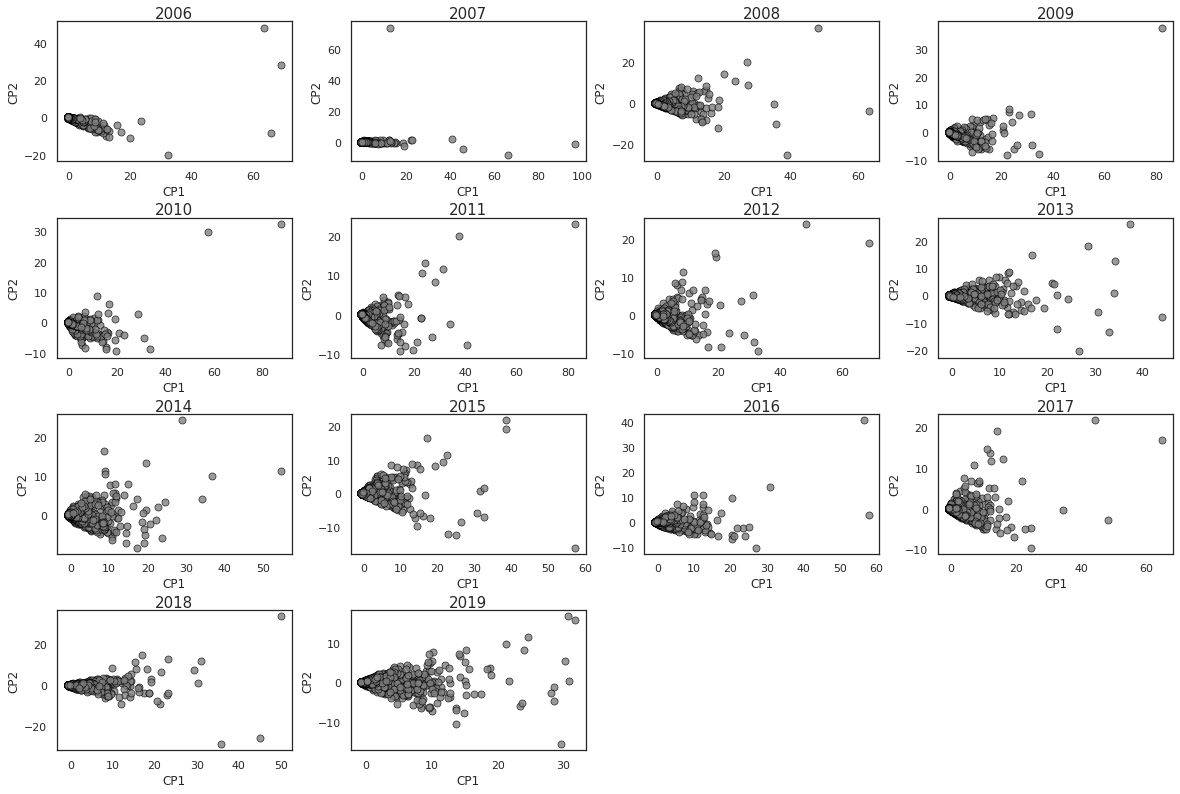
\includegraphics[width=1\textwidth]{figuras/cp1_cp2.png}
%	\caption{Diagrama de dispersão entre os dois primeiros componentes. Brasil $2006$ -- $2019$}
%	\small \textsuperscript {Fonte: Elaboração própria}
%    \label{corr_anos}
%\end{figure}

\begin{figure}[H]
	\centering
	\caption{Diagrama de dispersão entre os dois primeiros componentes. Brasil $2006$ -- $2019$}
	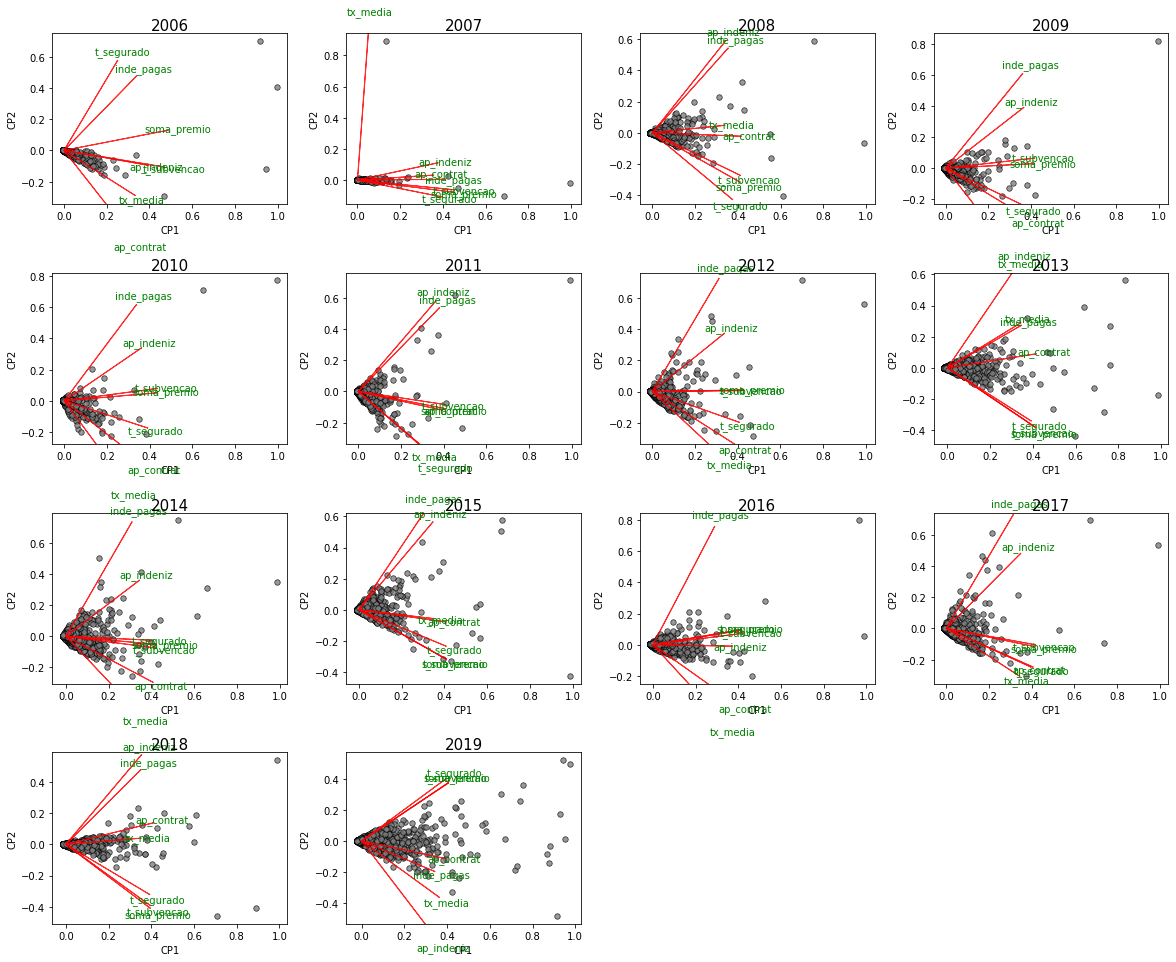
\includegraphics[width=1\textwidth]{figuras/acp_biplot.png}
	\small \textsuperscript {Fonte: Elaboração própria}
    \label{acp_biplot}
\end{figure}

\begin{figure}[H]
	\centering
	\caption{Correlação entre as variáveis de seguro Rural. Brasil $2006$ -- $2019$.}
	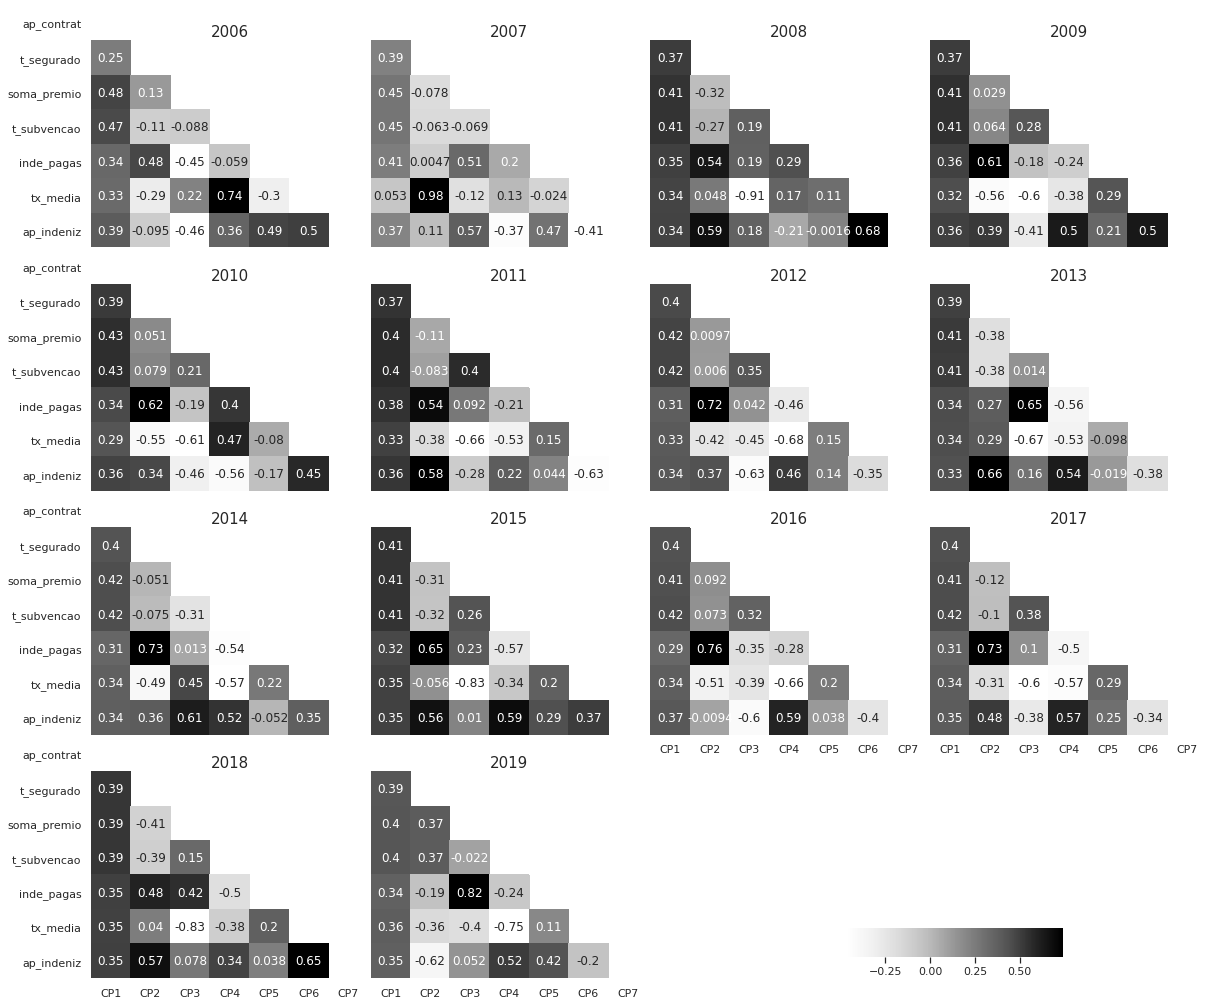
\includegraphics[width=0.9\textwidth]{figuras/corr_pca_var.png}
	\small \textsuperscript {Fonte: Elaboração própria.}
    \label{corr_pca_var}
\end{figure}

\subsection{ANÁLISE EXPLORATÓRIA DE DADOS ESPACIAIS}


\begin{figure}[H]
	\centering
	\caption{Distribuição espacial do primeiro componente principal. Brasil $2006$ -- $2019$.}
	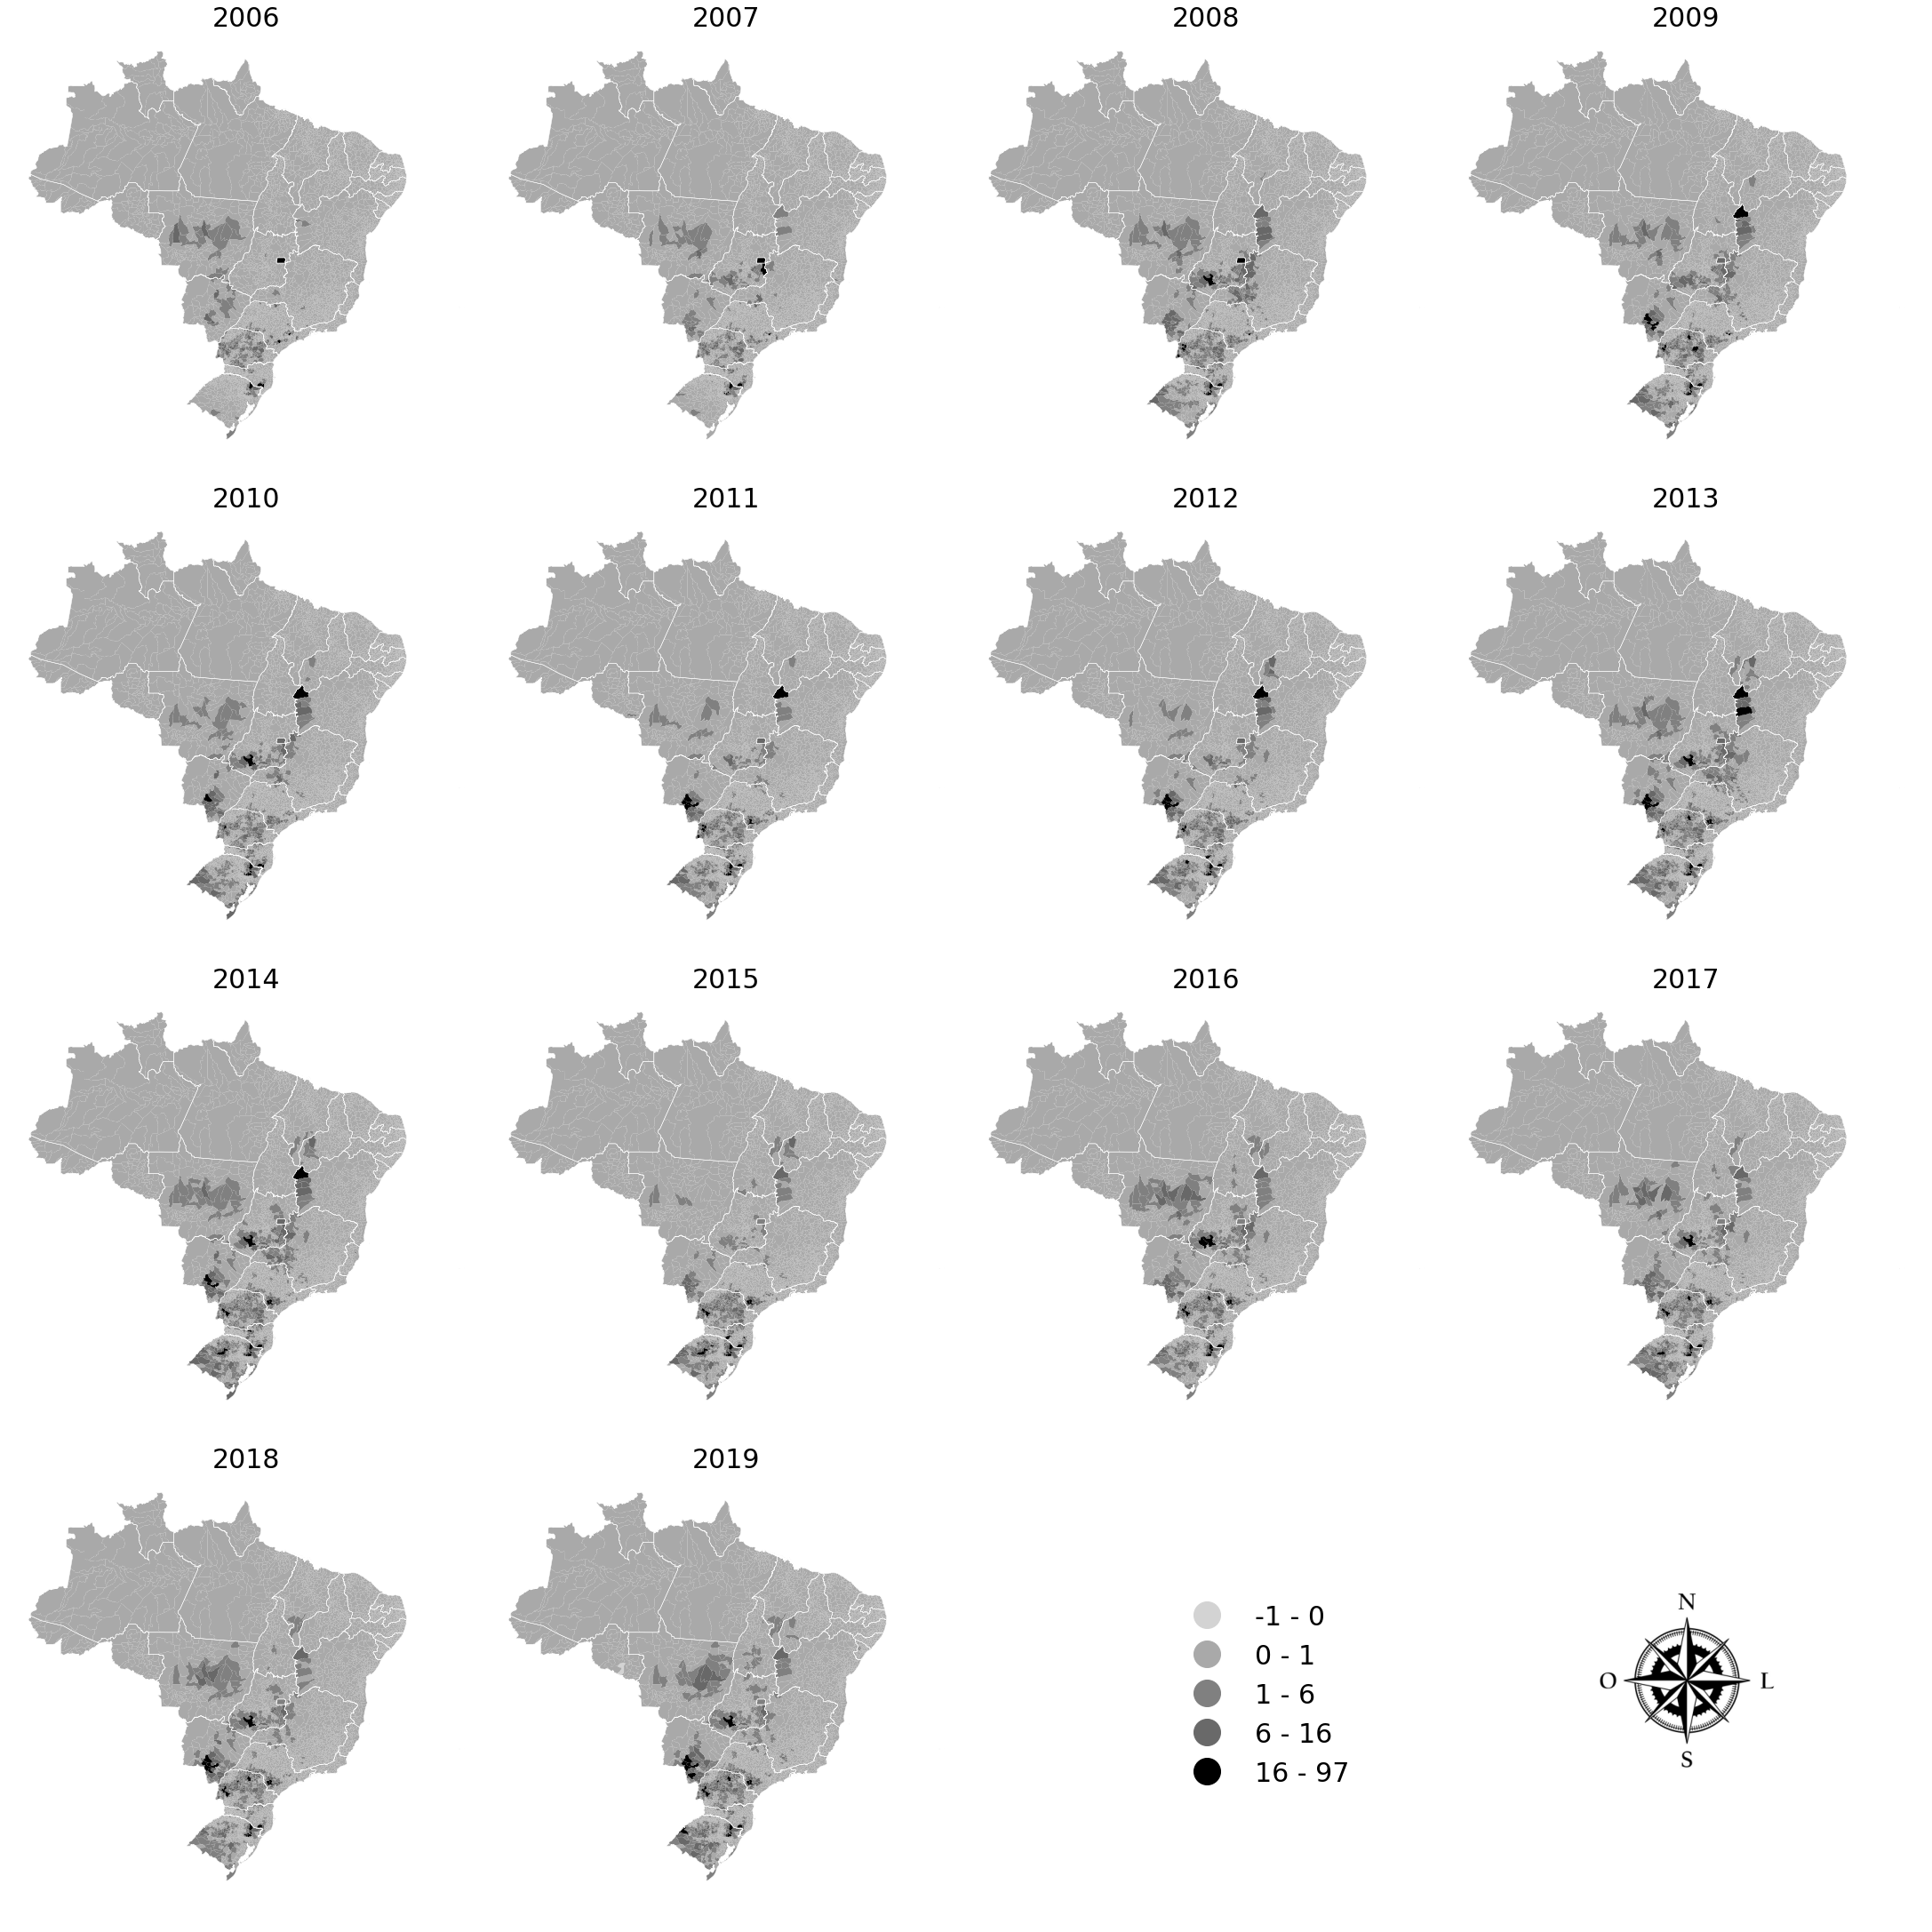
\includegraphics[width=0.9\textwidth]{figuras/map_CP1.png}\\
	\small \textsuperscript {Fonte: Elaboração própria.}
    \label{map_cp1}
\end{figure}

\begin{figure}[H]
	\centering
	\caption{Autocorrelação espacial (\textit{I} de Moran) do primeiro componente principal. Brasil $2006$ -- $2019$}
	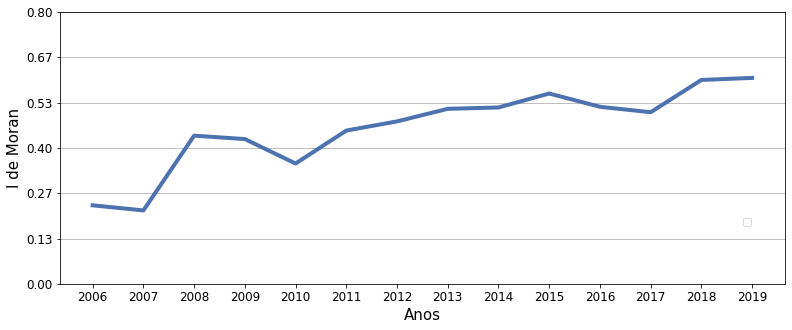
\includegraphics[width=0.8\textwidth]{figuras/i_de_moran_cp1.png}\\
	\small \textsuperscript {Fonte: Elaboração própria.}
    \label{i_moran_cp1}
\end{figure}


\begin{figure}[H]
	\centering
	\caption{Mapas \textit{LISA} para o primeiro componente principal.  Brasil $2006$ -- $2019$.}
	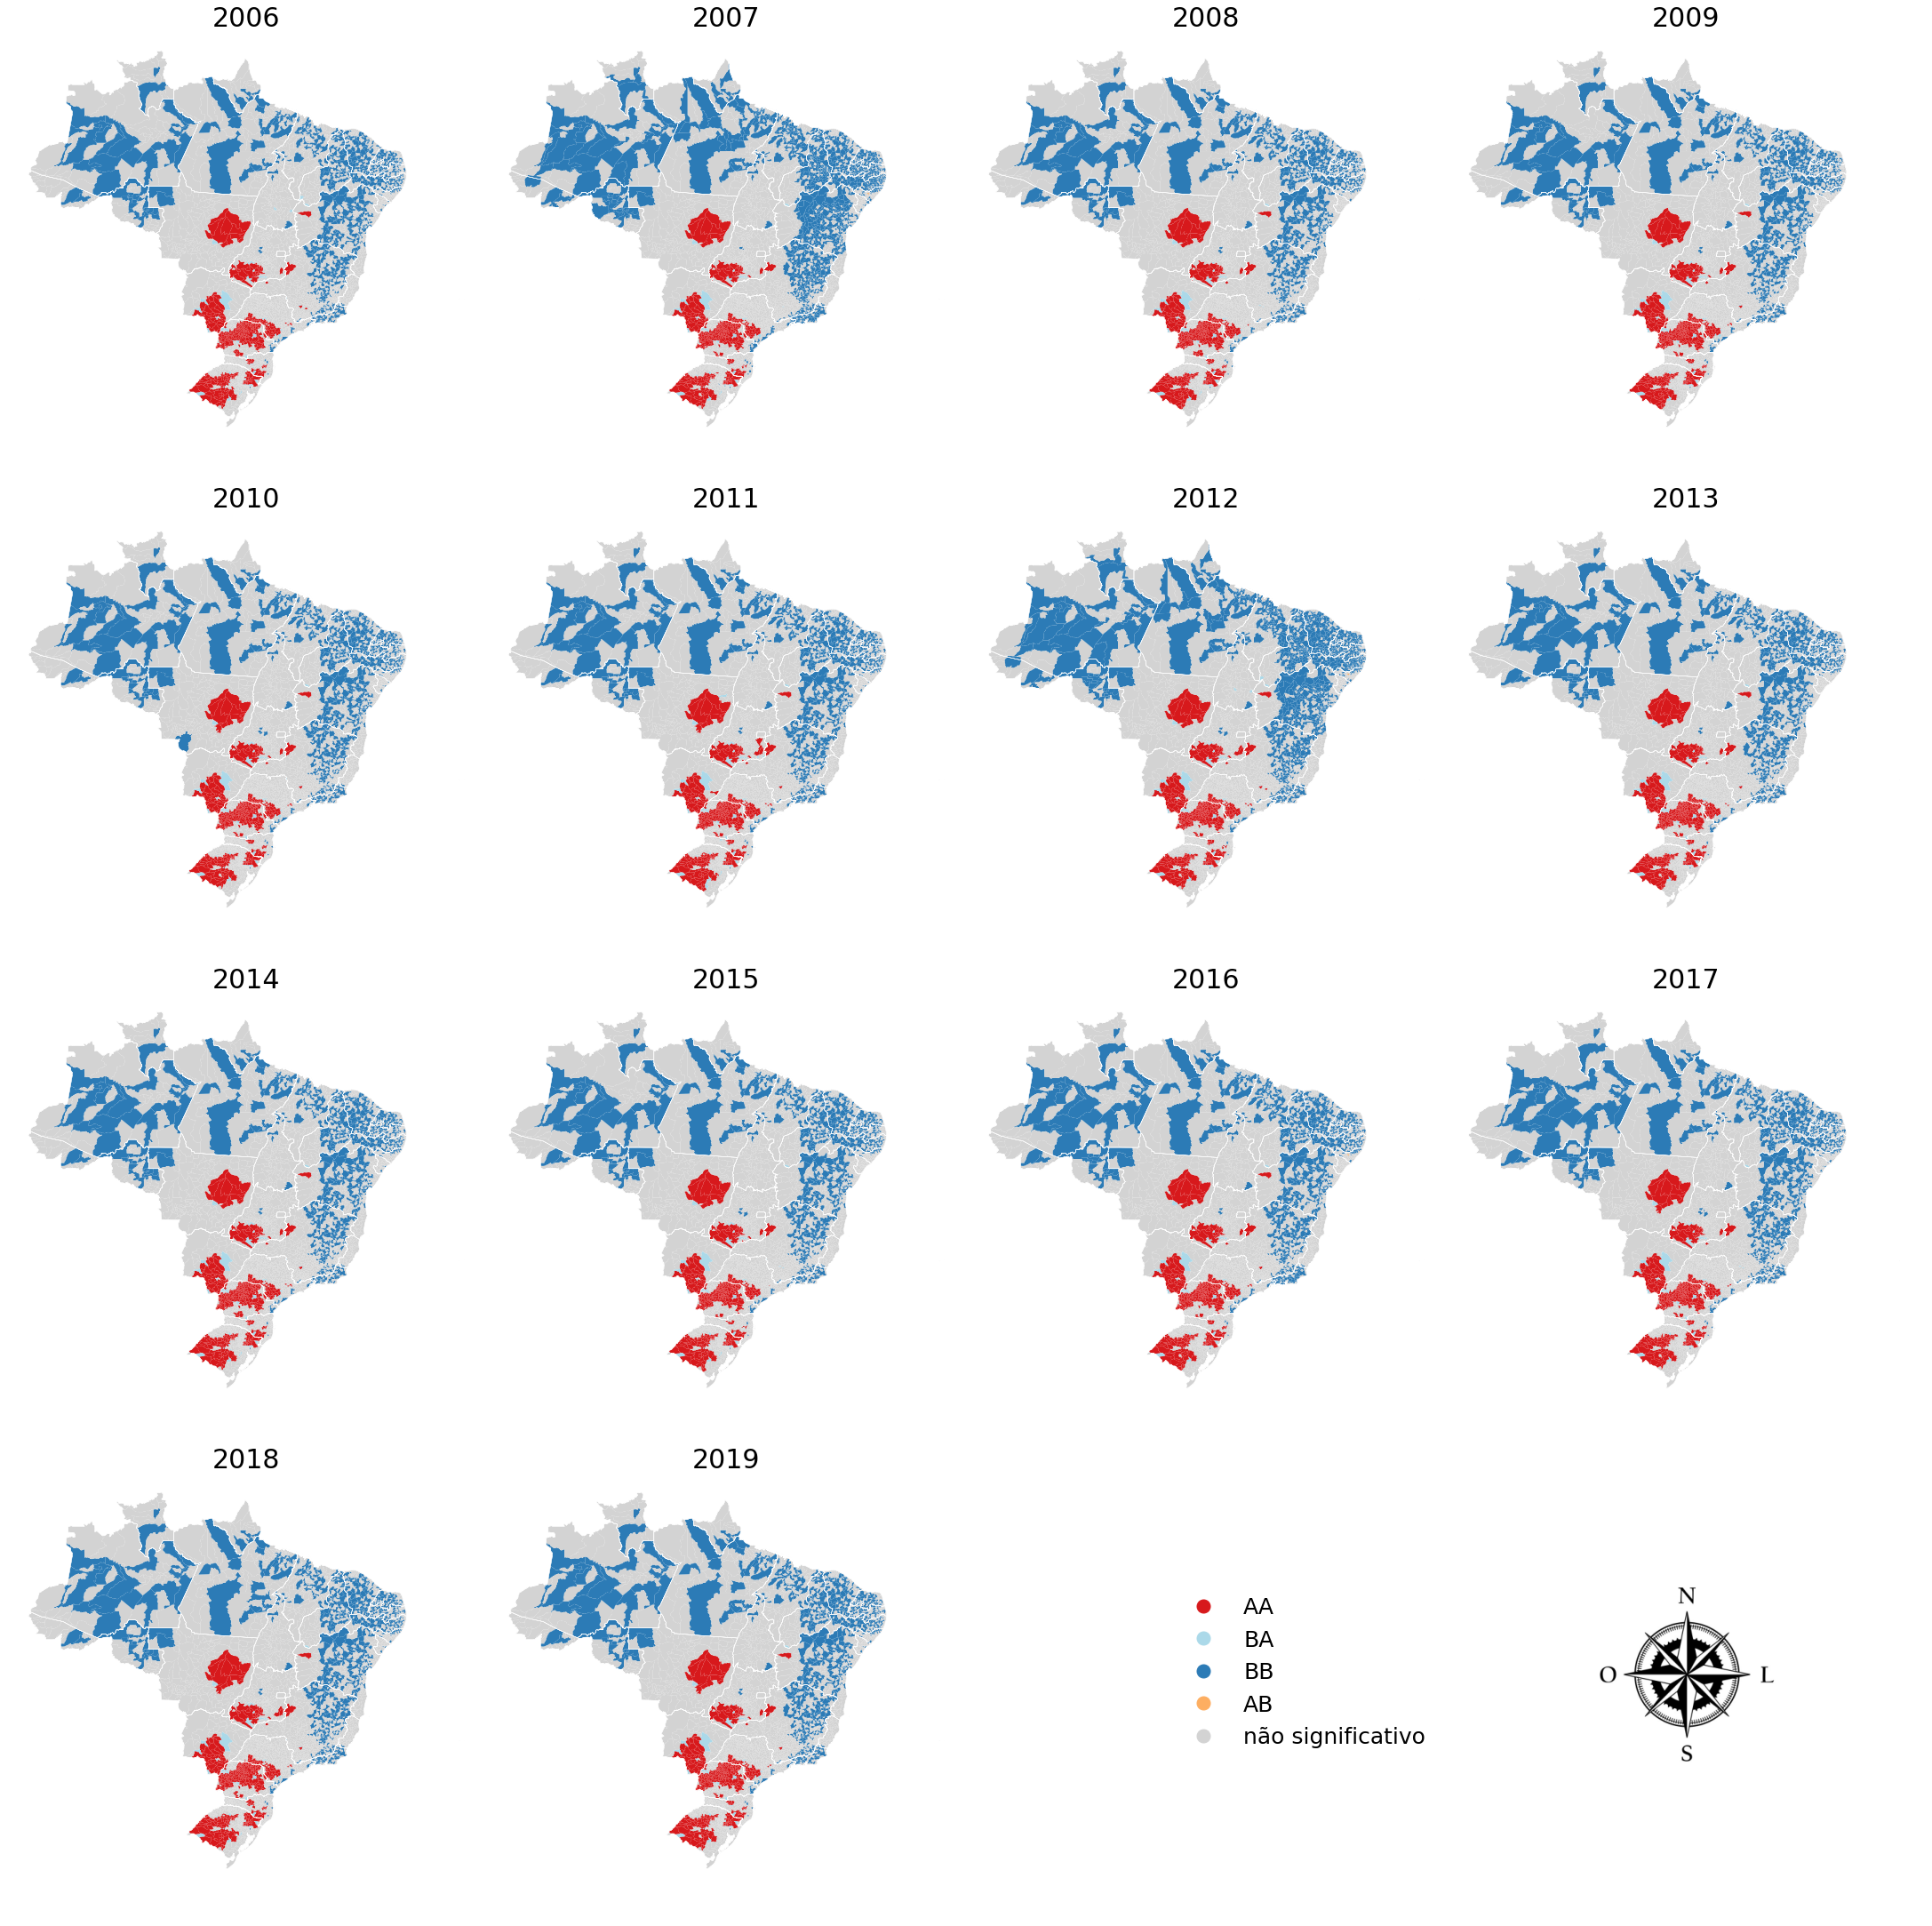
\includegraphics[width=0.9\textwidth]{figuras/map_lisa_cp1.png}\\
	\small \textsuperscript {Fonte: Elaboração própria.}
    \label{map_lisa_cp1}
\end{figure}

\section{CONSIDERAÇÕES FINAIS}\label{sc-conclusion}

\newpage
\addcontentsline{toc}{section}{\hspace*{\distnumber}REFERÊNCIAS}
\begin{center}
\section*{REFERÊNCIAS} 
\end{center}

    
% Use isso descomentado durante edição.
% Quando concluir a Tese, comente iss e use
% o código do bloco abaixo.
%\begin{singlespace}
%\renewcommand\refname{}
%\begin{flushleft}
%\bibliography{../tese/bibtese2}
%\end{flushleft}
%\end{singlespace}

%% Em cap2nlme-corrigido.bbl foi feita correção manual de
%% algumas referências como por exemplo as citações
%% de Dissertação e Tese.
%% Então deixa-se de usar o arquivo cap2nlme.bbl gerado
%% automaticamente pelo abntcite, mas isso é só ao final.
\begin{singlespace}
\begin{flushleft}
\renewcommand\refname{}
\vspace*{-1.5cm}
%==========================================================================================

\documentclass[10pt]{article}

%==========================================================================================

\usepackage[utf8]{inputenc}
\usepackage[brazil]{babel}
\usepackage[T1]{fontenc}
\usepackage{amsmath}
\usepackage{amsfonts}
\usepackage{mathrsfs}
\usepackage{amssymb}
\usepackage{graphicx}
\usepackage{geometry, calc, color, setspace}
\usepackage{indentfirst}
\usepackage{wrapfig}
\usepackage{boxedminipage}
\usepackage{enumerate}
\usepackage{float}
\usepackage{paralist}
\usepackage{comment}
\usepackage{icomma}
\usepackage{rotating}
\usepackage{multirow}
\usepackage[position=bottom]{subfig}
\usepackage{array}
\usepackage{tabularx}
\usepackage{float}
\usepackage{array}

\newcolumntype{L}[1]{>{\raggedright\let\newline\\\arraybackslash\hspace{0pt}}m{#1}}
\newcolumntype{C}[1]{>{\centering\let\newline\\\arraybackslash\hspace{0pt}}m{#1}}
%\newcolumntype{R}[1]{>{\raggedleft\let\newline\\\arraybackslash\hspace{0pt}}m{#1}}
\newcolumntype{R}{>{\raggedleft\let\newline\\\arraybackslash\hspace{0pt}}X}

\usepackage[alf,bibjustif]{abntex2cite}
%\usepackage{abntcite}

% Para o alinhamento dos títulos das figuras
\usepackage{caption}
%\captionsetup[figure]{format=hang,labelsep=endash,font=small,justification=RaggedRight,singlelinecheck=off, margin=1cm}
\captionsetup[subfigure]{textfont=small,singlelinecheck=off,justification=raggedright}


%%  Inserindo os códigos Python ==================================
\usepackage{listings}

%\definecolor{light_gray}{rgb}{0.97,0.97,0.97}
%\definecolor{mymauve}{rgb}{0.58,0,0.82}
%\definecolor{mygreen}{rgb}{0,0.6,0}

\lstset{
  language = Python,
  inputencoding = utf8,
  backgroundcolor = \color{white},
  columns=fullflexible,
  basicstyle=\ttfamily,
  breaklines=true,
  postbreak=\raisebox{0ex}[0ex][0ex]{\color{black}$\hookrightarrow$\space},
  keywordstyle=\color{black},      % keyword style
  stringstyle=\color{black},
  commentstyle=\color{black}
}

\newcommand{\HRule}{\noindent\rule{\linewidth}{0.2mm}}

\usepackage{mathpazo}                         % tem suporte matemático
\usepackage[scaled=0.85]{beramono}            % usa esta nos verbatins [scaled=0.9]

\renewcommand\UrlFont{\color{black}\rmfamily} 

\def\distnumber{2.3em}

%==========================================================================================

\author{Walef Machado de Mendonça\footnote{Mestrando em Estatística Aplicada e Biometria na Universidade Federal de Alfenas}\\
Patrícia de Siqueira Ramos\footnote{Professora da Universidade Federal de Alfenas, campus Varginha}}

%==========================================================================================


\title{Análise de autocorrelação espacial de dados multivariados de seguro rural}
\date{}

\begin{document}

\maketitle

\begin{abstract}
\noindent O ambiente no qual se desenvolvem as atividades agropecuárias apresenta elevado risco e grande incerteza. Diversos fatores relacionados ao setor agropecuário podem gerar oscilações na renda dos produtores. Estas oscilações devem ser enfrentadas por meio de políticas de apoio à gestão de riscos como, por exemplo, a contratação de seguro rural. Esta modalidade de seguro possibilita a recuperação da capacidade financeira do produtor na ocorrência de eventos adversos que causem prejuízo econômico. Considerando a relevância do seguro rural no setor agropecuário, este trabalho tem como objetivo avaliar a distribuição espacial das variáveis desse seguro nos municípios brasileiros no período de 2006 a 2019. Para alcançar tal objetivo, foi utilizada a Análise de Componentes Principais, com o objetivo de reduzir a dimensionalidade dos dados e a Análise Exploratória de Dados Espaciais para investigar a presença de padrões de distribuição espacial do seguro rural. Os dados utilizados são provenientes dos censos do seguro rural, compilados pelo Ministério da Agricultura, Pecuária e Abastecimento. Com a utilização de escores dos CPs, verificou-se que as maiores concentrações de apólices de seguro rural estão situadas nas regiões Sul e Centro-Oeste e há uma tendência de aumento na dependência espacial do seguro rural ao longo do período analisado. \\
\newline
\noindent {\textbf{Palavras-chave}}: Seguro rural. Política agrícola. Estatística espacial. Autocorrelação espacial. I de Moran.
\end{abstract}


\section{INTRODUÇÃO}

As atividades agropecuárias têm grande relevância na economia brasileira. Segundo um estudo realizado pelo Centro de Estudos Avançados em Economia Aplicada (CEPEA), da Esalq/USP, a parcela da participação do agronegócio no PIB brasileiro foi de $20,5\%$ em $2019$, e em $2020$, este percentual chegou à $26,6\%$ \cite{cepea21_2}. De acordo com o último Censo Agropecuário, entre $2006$ e $2017$, houve um acréscimo de cerca de $5,8\%$ na área total dos estabelecimentos agropecuários e, tanto a área total quanto a produção agrícola e pecuária apresentaram um considerável crescimento \cite{ibge19_2}.

No entanto, o ambiente no qual se desenvolvem as atividades agropecuárias apresenta elevado risco e significativa incerteza. Essa insegurança se deve, principalmente, às instabilidades climáticas e ameaças sanitárias, que podem afetar a produção, ou à razões de mercado, como variações das taxas de câmbio e juros, ou a condições ligadas ao ambiente de negócios, tais como alterações em marcos regulatórios e em políticas públicas. Todas essas variáveis, relacionadas aos mercados agropecuários, geram variações na renda do setor, que são comumente enfrentadas por meio de políticas de apoio à gestão de riscos \cite{brasil18_2}.

O gerenciamento de riscos agropecuários pode ocorrer de diversas maneiras. No entanto, a contratação de seguro rural é uma das formas mais usuais. Essa modalidade de seguro atua no sentido de amenizar as perdas e possibilitar a recuperação da capacidade financeira do produtor na ocorrência de sinistros. O seguro rural propicia um ambiente mais favorável ao desenvolvimento das atividades agropecuárias, pois proporciona a garantia do fluxo de renda, favorece um aumento da área plantada e facilita a obtenção de financiamento. Além disso, se mostra um instrumento que possibilita o compartilhamento do risco da agropecuária com outros agentes e setores econômicos \cite{brasil19_2}.

%É importante destacar que o mercado de seguro rural não se consolida sem a participação do Estado. Destacam-se problemas como os elevados investimentos e custos administrativos, a possibilidade de riscos catastróficos, a forte influência do risco moral e da seleção adversa na formação das carteiras, como fatores que limitam a eficiência da iniciativa privada na oferta de produtos. Nesse sentido, o poder público é demandado a interferir no mercado, seja atuando diretamente como seguradora, seja criando programas que estimulem a oferta e a demanda por produtos de seguro (BRASIL, 2019a). 

% Esses dois estão ok...

Considerando a relevância do seguro rural no setor agropecuário, este estudo tem como objetivo analisar a distribuição espacial de dados multivariados do seguro rural nos municípios brasileiros entre os anos de $2006$ e $2019$. Além disso, busca-se investigar a presença de padrões de distribuição espacial nos dados, mais especificamente, se há presença de dependência ou heterogeneidade espacial. Por fim, este trabalho pretende fornecer informações que possam contribuir para o debate em torno do aperfeiçoamento do sistema de seguro rural no Brasil. Para alcançar tais objetivos, o trabalho faz uso da Análise de Componentes Principais (ACP) para reduzir a dimensionalidade dos dados e da Análise Exploratória de Dados Espaciais (AEDE), para investigar a presença de padrões de distribuição espacial. São utilizados dados oriundos dos Censos do Seguro Rural, compilados pelo Ministério da Agricultura, Pecuária e Abastecimento \cite{brasil21}.

O trabalho estrutura-se da seguinte forma: na seção $2$ é apresentado uma revisão de literatura a respeito do seguro rural no Brasil, assim como a Análise de Componentes Principais e a Análise Exploratória de Dados Espaciais. A seção $3$ descreve a metodologia utilizada neste estudo, a fonte dos dados e os recursos computacionais. A seção $4$ discute os resultados obtidos. Por fim, a seção $5$ traz as considerações finais. 


%Ao longo dos últimos anos, o agronegócio tem sido o único setor da economia brasileira que vem mantendo crescimento. Esse resultado é fruto do aumento na área plantada com as principais culturas, e, principalmente, dos investimentos em máquinas, equipamentos e tecnologias e, em consequência, do aumento da produtividade no campo.

%Apesar desses resultados positivos, mesmo em anos de safras recordes, eventos climáticos de abrangência regional têm afetado os produtores, causando perdas significativas em suas lavouras e na sua rentabilidade

%\section{REFERENCIAL TEÓRICO}\label{referencial}

\section{MATERIAL E MÉTODOS}\label{methods}

Nesse trabalho, foi utilizada a análise exploratória de dados espaciais com o objetivo de avaliar a distribuição espacial do seguro rural nos municípios brasileiros no período de $2006$ a $2019$. Inicialmente, foi realizada uma análise exploratória dos dados de forma a auxiliar a análise de componentes principais e análise exploratória espacial. O resumo estatístico das variáveis estudadas foi obtido e, de modo a identificar os pares de variáveis mais associadas entre si, foram calculadas as matrizes de correlações de Pearson entre as variáveis, para cada um dos anos entre $2006$ e $2019$. A matriz de correlações linear tem a forma apresentada na definição (\ref{def_matriz_corr_2}).

Após a análise exploratória, foi empregada a análise de componentes principais (ACP) com o objetivo de reduzir a dimensionalidade dos dados. O método foi aplicado com a intenção de reduzir o conjunto das variáveis originais correlacionadas entre si a um novo conjunto de variáveis, os componentes principais (CPs), não correlacionadas. Os escores, valores numéricos dos componentes, do primeiro componente principal (CP1) foram utilizados para a análise exploratória de dados espaciais (AEDE). 

Para a realização da AEDE, é necessária a utilização da matriz de pesos espaciais apresentada na subseção \ref{W_matrix_2}. Para a construção dessa matriz de pesos espaciais, foram desconsiderados os municípios de Fernando de Noronha (PE) e Ilhabela (SP). Esses municípios foram retirados da análise pois, além de se constituírem de ilhas, não possuem nenhuma apólice de seguro rural contratada durante os anos analisados. 

% Dados
Foram utilizados dados anuais referentes a apólices de seguro rural dos municípios brasileiros a partir do ano de $2006$ até o ano de $2019$ (último ano disponível até então). As variáveis utilizadas na análise são apresentadas na Tabela \ref{tab_variaveis}. Para todas as variáveis, foi utilizado o nível de agregação municipal. Nos casos em que as informações disponíveis eram referentes a outras localidades, como distritos, fazendas e vilarejos, tais informações foram atribuídas aos municípios correspondentes. 

\begin{small}
\begin{table}[!htp]
\caption{Descrição das variáveis utilizadas.}\label{tab_variaveis}
 \input{../anexos/variaveis.tex}
\end{table}
\end{small}
	
% Fonte dos Dados 
Os dados sobre seguro rural estão disponíveis no endereço eletrônico do Ministério da Agricultura, Pecuária e Abastecimento (MAPA). Os dados que contém atributos geográficos, como a posição e o formato, do território brasileiro estão disponíveis no endereço eletrônico do Instituto Brasileiro de Geografia e Estatística (IBGE, 2020).
	
%Padronização
Como as variáveis estão em diferentes escalas e, com isto, possuem diferentes variâncias, foi realizada a padronização das variáveis para que tais fatores não interferissem na análise. Tal padronização foi efetuada subtraindo-se de cada observação a média de sua respectiva variável e dividindo-se posteriormente pelo desvio padrão da variável.

% Linguagem de programação 
Esse estudo foi realizado com a linguagem de programação \textit{Python} \cite{python17_2}, utilizando-se a interface \textit{Jupyter} \cite{jupyter17_2}, \cite{perez07_2} \cite{kluyver19_2}.
Além disso, as seguintes bibliotecas foram utilizadas: 
\textit{Pandas} \cite{mckinney10_2}, para a manipulação de dados,
\textit{NumPy} \cite{walt11_2}, que possibilita computação numérica com \textit{Python},
\textit{Matplotlib} \cite{hunter07_2} e \textit{Seaborn} \cite{waskom14_2}, que são bibliotecas para a criação de gráficos,
\textit{jenkspy} para a utilização do algoritmo Fisher Jenks \cite{jenks77_2}. 
A análise de componentes principais foi realizada através da biblioteca \textit{sklearn} e as bibliotecas \textit{Geopandas} \cite{jordahl14_2} e \textit{PySAL} \cite{rey07_2} possibilitaram a análise espacial.

% Fisher-Jenks. Tal método, segundo \citeonline{rey2013}, é frequentemente recomendado por cartógrafos, sendo apresentado por \citeonline{jenks1977} e originalmente proposto por \citeonline{fisher1958}, a abordagem baseia-se no particionamento ideal de dados univariados. 

%@article{rey2013,
%  title={Parallel optimal choropleth map classification in PySAL},
%  author={Rey, Sergio and Anselin, Luc and Pahle, Robert and Kang, Xing and Stephens, Philip},
%  journal={International Journal of Geographical Information Science},
%  volume={27},
%  number={5},
%  pages={1023--1039},
%  year={2013},
%  publisher={Taylor \& Francis}
%}

%@article{fisher1958,
%  title={On grouping for maximum homogeneity},
%  author={Fisher, Walter},
%  journal={Journal of the American statistical Association},
%  volume={53},
%  number={284},
%  pages={789--798},
%  year={1958},
%  publisher={Taylor \& Francis}
%}

%@article{jenks1977,
%  title={Optimal data classification for choropleth maps},
%  author={Jenks, George},
%  journal={Department of Geography, University of Kansas Occasional Paper},
%  year={1977}
%}


\section{RESULTADOS E DISCUSSÃO}\label{sc-results}

\subsection{CORRELAÇÃO ENTRE AS VARIÁVEIS} 

A Figura \ref{corr_anos} apresenta os valores das correlações de Pearson entre cada um dos pares de variáveis de seguro rural utilizadas. Quanto mais escura a cor do retângulo mais próximo de $1$ é o valor do coeficiente de correlação e, portanto, maior o grau de associação entre as variáveis. Por outro lado, quanto mais clara a cor do retângulo, mais próximo de $0$ é o valor do coeficiente de correlação e, portanto, menor o grau de associação entre as variáveis\footnote{Esta representação com escala em cinza foi escolhida por não haver, nos dados analisados, a presença de correlação negativa.}.

\begin{figure}[H]
	\centering
	\caption{Correlação entre as variáveis de seguro Rural. Brasil $2006$ -- $2019$}
	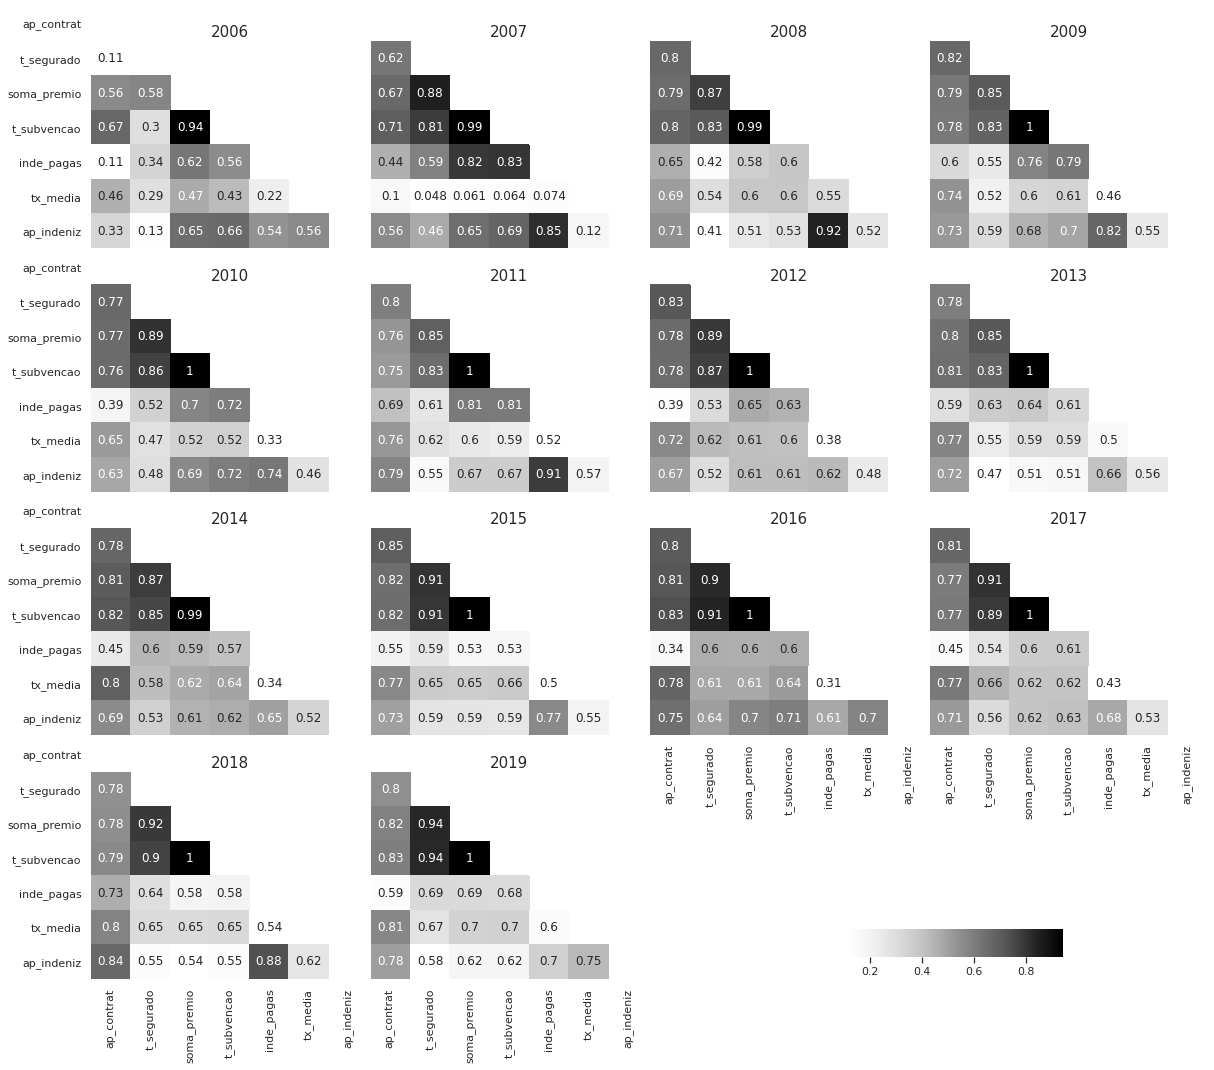
\includegraphics[width=0.9\textwidth]{figuras/corr_anos_bw.png}
	\parbox{\dimexpr\linewidth-2cm}{\raggedright
    \strut \textsuperscript{Fonte: Elaboração própria}\strut}
    \label{corr_anos}
\end{figure}

\subsection{ANÁLISE DE COMPONENTES PRINCIPAIS} 

\begin{small}
\begin{table}[H]
\caption{Proporção da variância explicada acumulada pelos componentes principais. Brasil $2006$ -- $2019$} \label{tab_var_ratio}
\input{../anexos/var_ratio.tex}
\end{table}
\end{small}


\begin{figure}[H]
	\centering
	\caption{Variância explicada acumulada pelos componentes principais. Brasil $2006$ -- $2019$}
	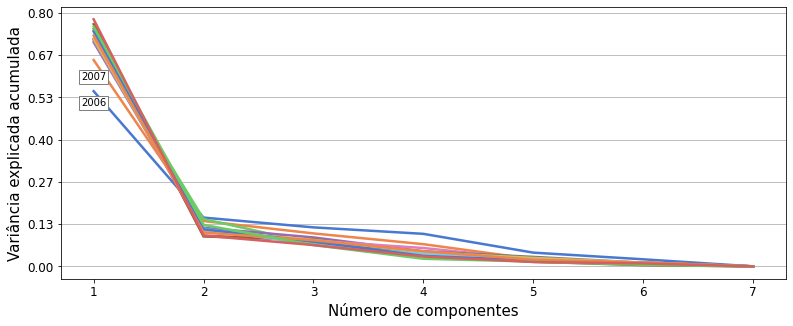
\includegraphics[width=0.8\textwidth]{figuras/var_radio.png}\\
	\small \textsuperscript {Fonte: Elaboração própria}
    \label{var_ratio}
\end{figure}

Devido à estrutura de correlação entre as variáveis de seguro rural foi possível utilizar os escores do primeiro componente principal como uma variável representativa das demais variáveis originais. A correlação dos escores do primeiro componente principal foram, em todos os anos, positivamente correlacionados com todas as variáveis originais. Além disso, em todos os anos analisados, a variância explicada acumulada pelo primeiro componente foi superior à $55,3\%$. 

%\begin{figure}[H]
%	\centering
%	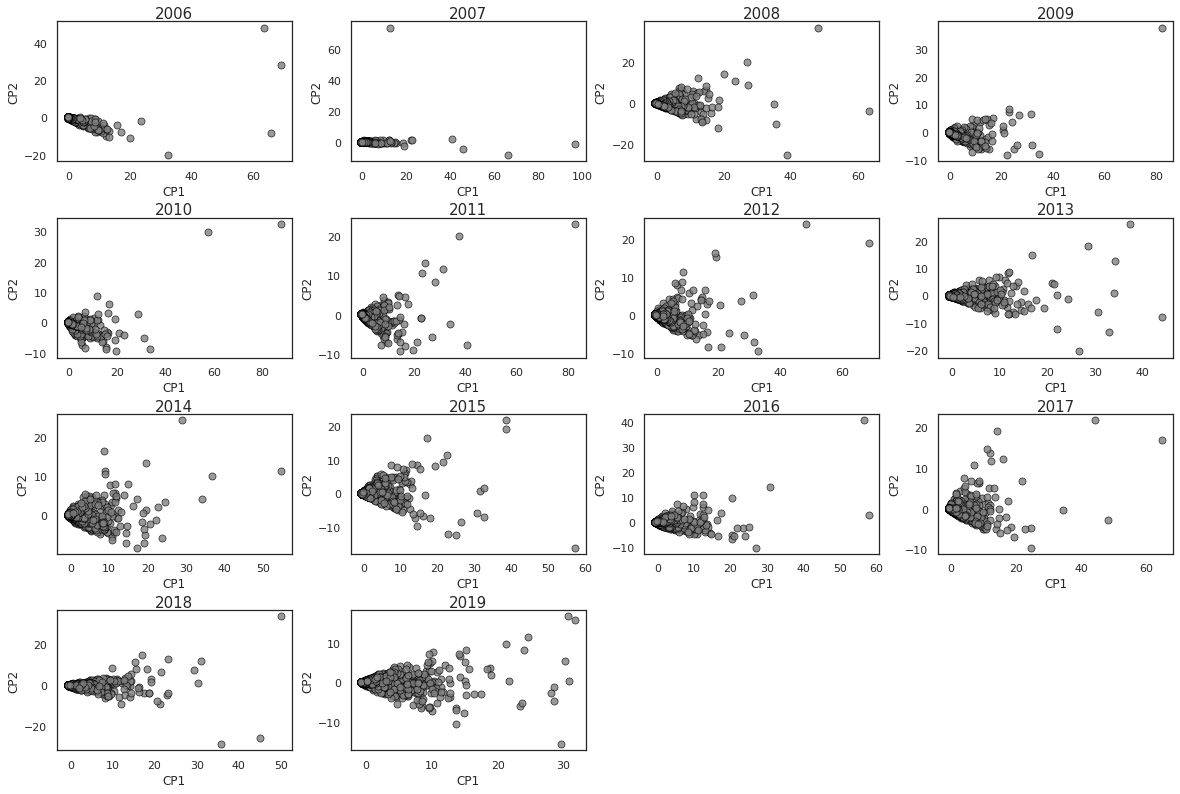
\includegraphics[width=1\textwidth]{figuras/cp1_cp2.png}
%	\caption{Diagrama de dispersão entre os dois primeiros componentes. Brasil $2006$ -- $2019$}
%	\small \textsuperscript {Fonte: Elaboração própria}
%    \label{corr_anos}
%\end{figure}

\begin{figure}[H]
	\centering
	\caption{Diagrama de dispersão entre os dois primeiros componentes. Brasil $2006$ -- $2019$}
	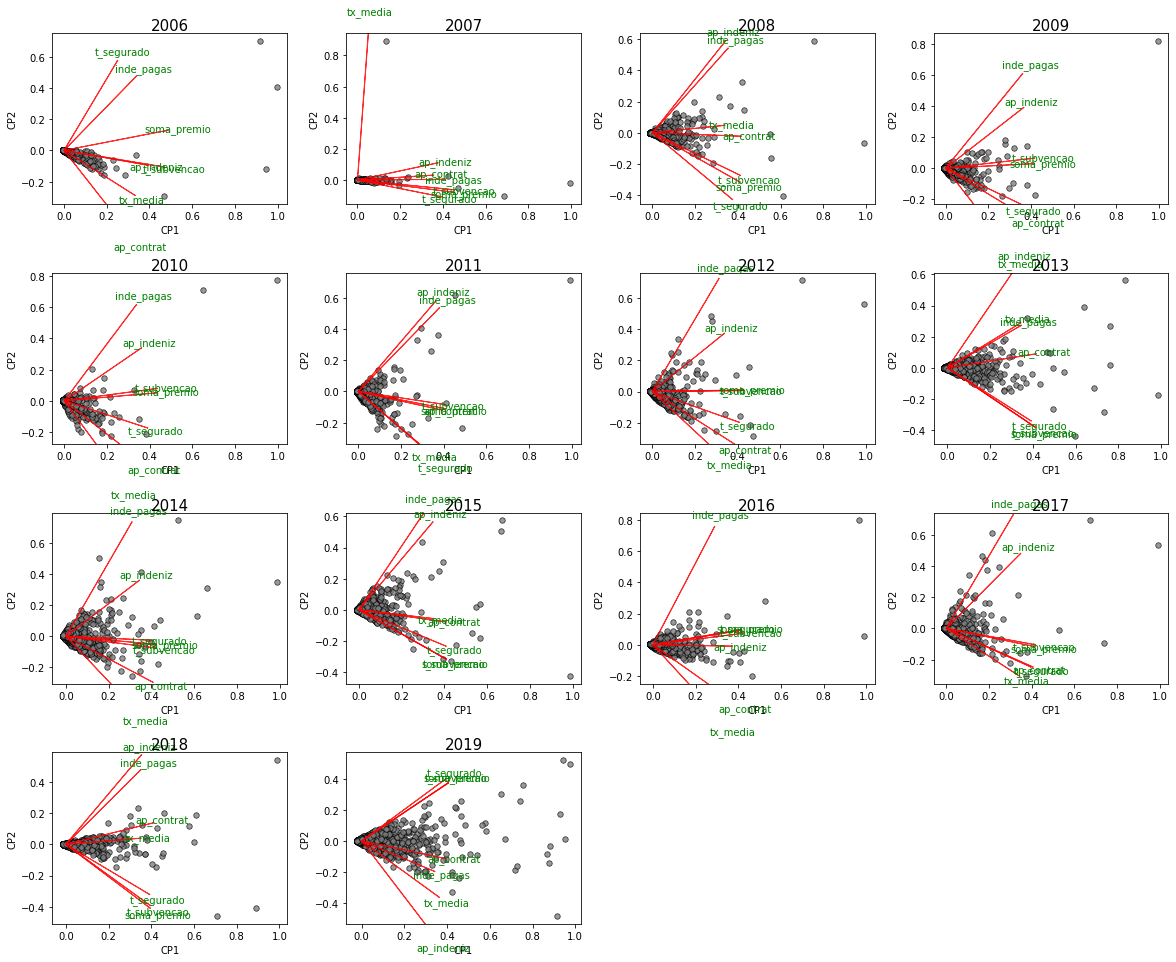
\includegraphics[width=1\textwidth]{figuras/acp_biplot.png}
	\small \textsuperscript {Fonte: Elaboração própria}
    \label{acp_biplot}
\end{figure}

\begin{figure}[H]
	\centering
	\caption{Correlação entre as variáveis de seguro Rural. Brasil $2006$ -- $2019$.}
	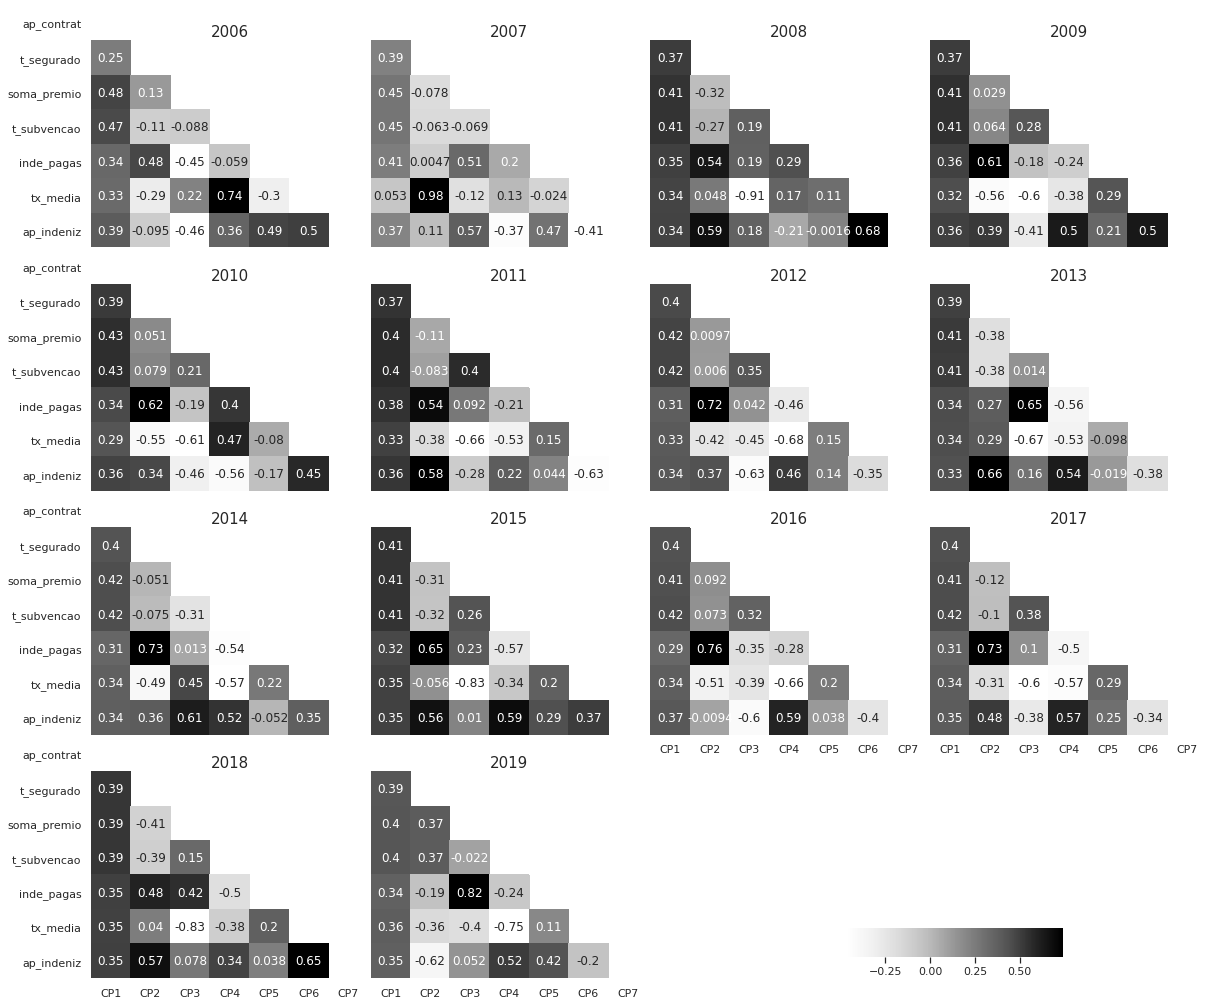
\includegraphics[width=0.9\textwidth]{figuras/corr_pca_var.png}
	\small \textsuperscript {Fonte: Elaboração própria.}
    \label{corr_pca_var}
\end{figure}

\subsection{ANÁLISE EXPLORATÓRIA DE DADOS ESPACIAIS}


\begin{figure}[H]
	\centering
	\caption{Distribuição espacial do primeiro componente principal. Brasil $2006$ -- $2019$.}
	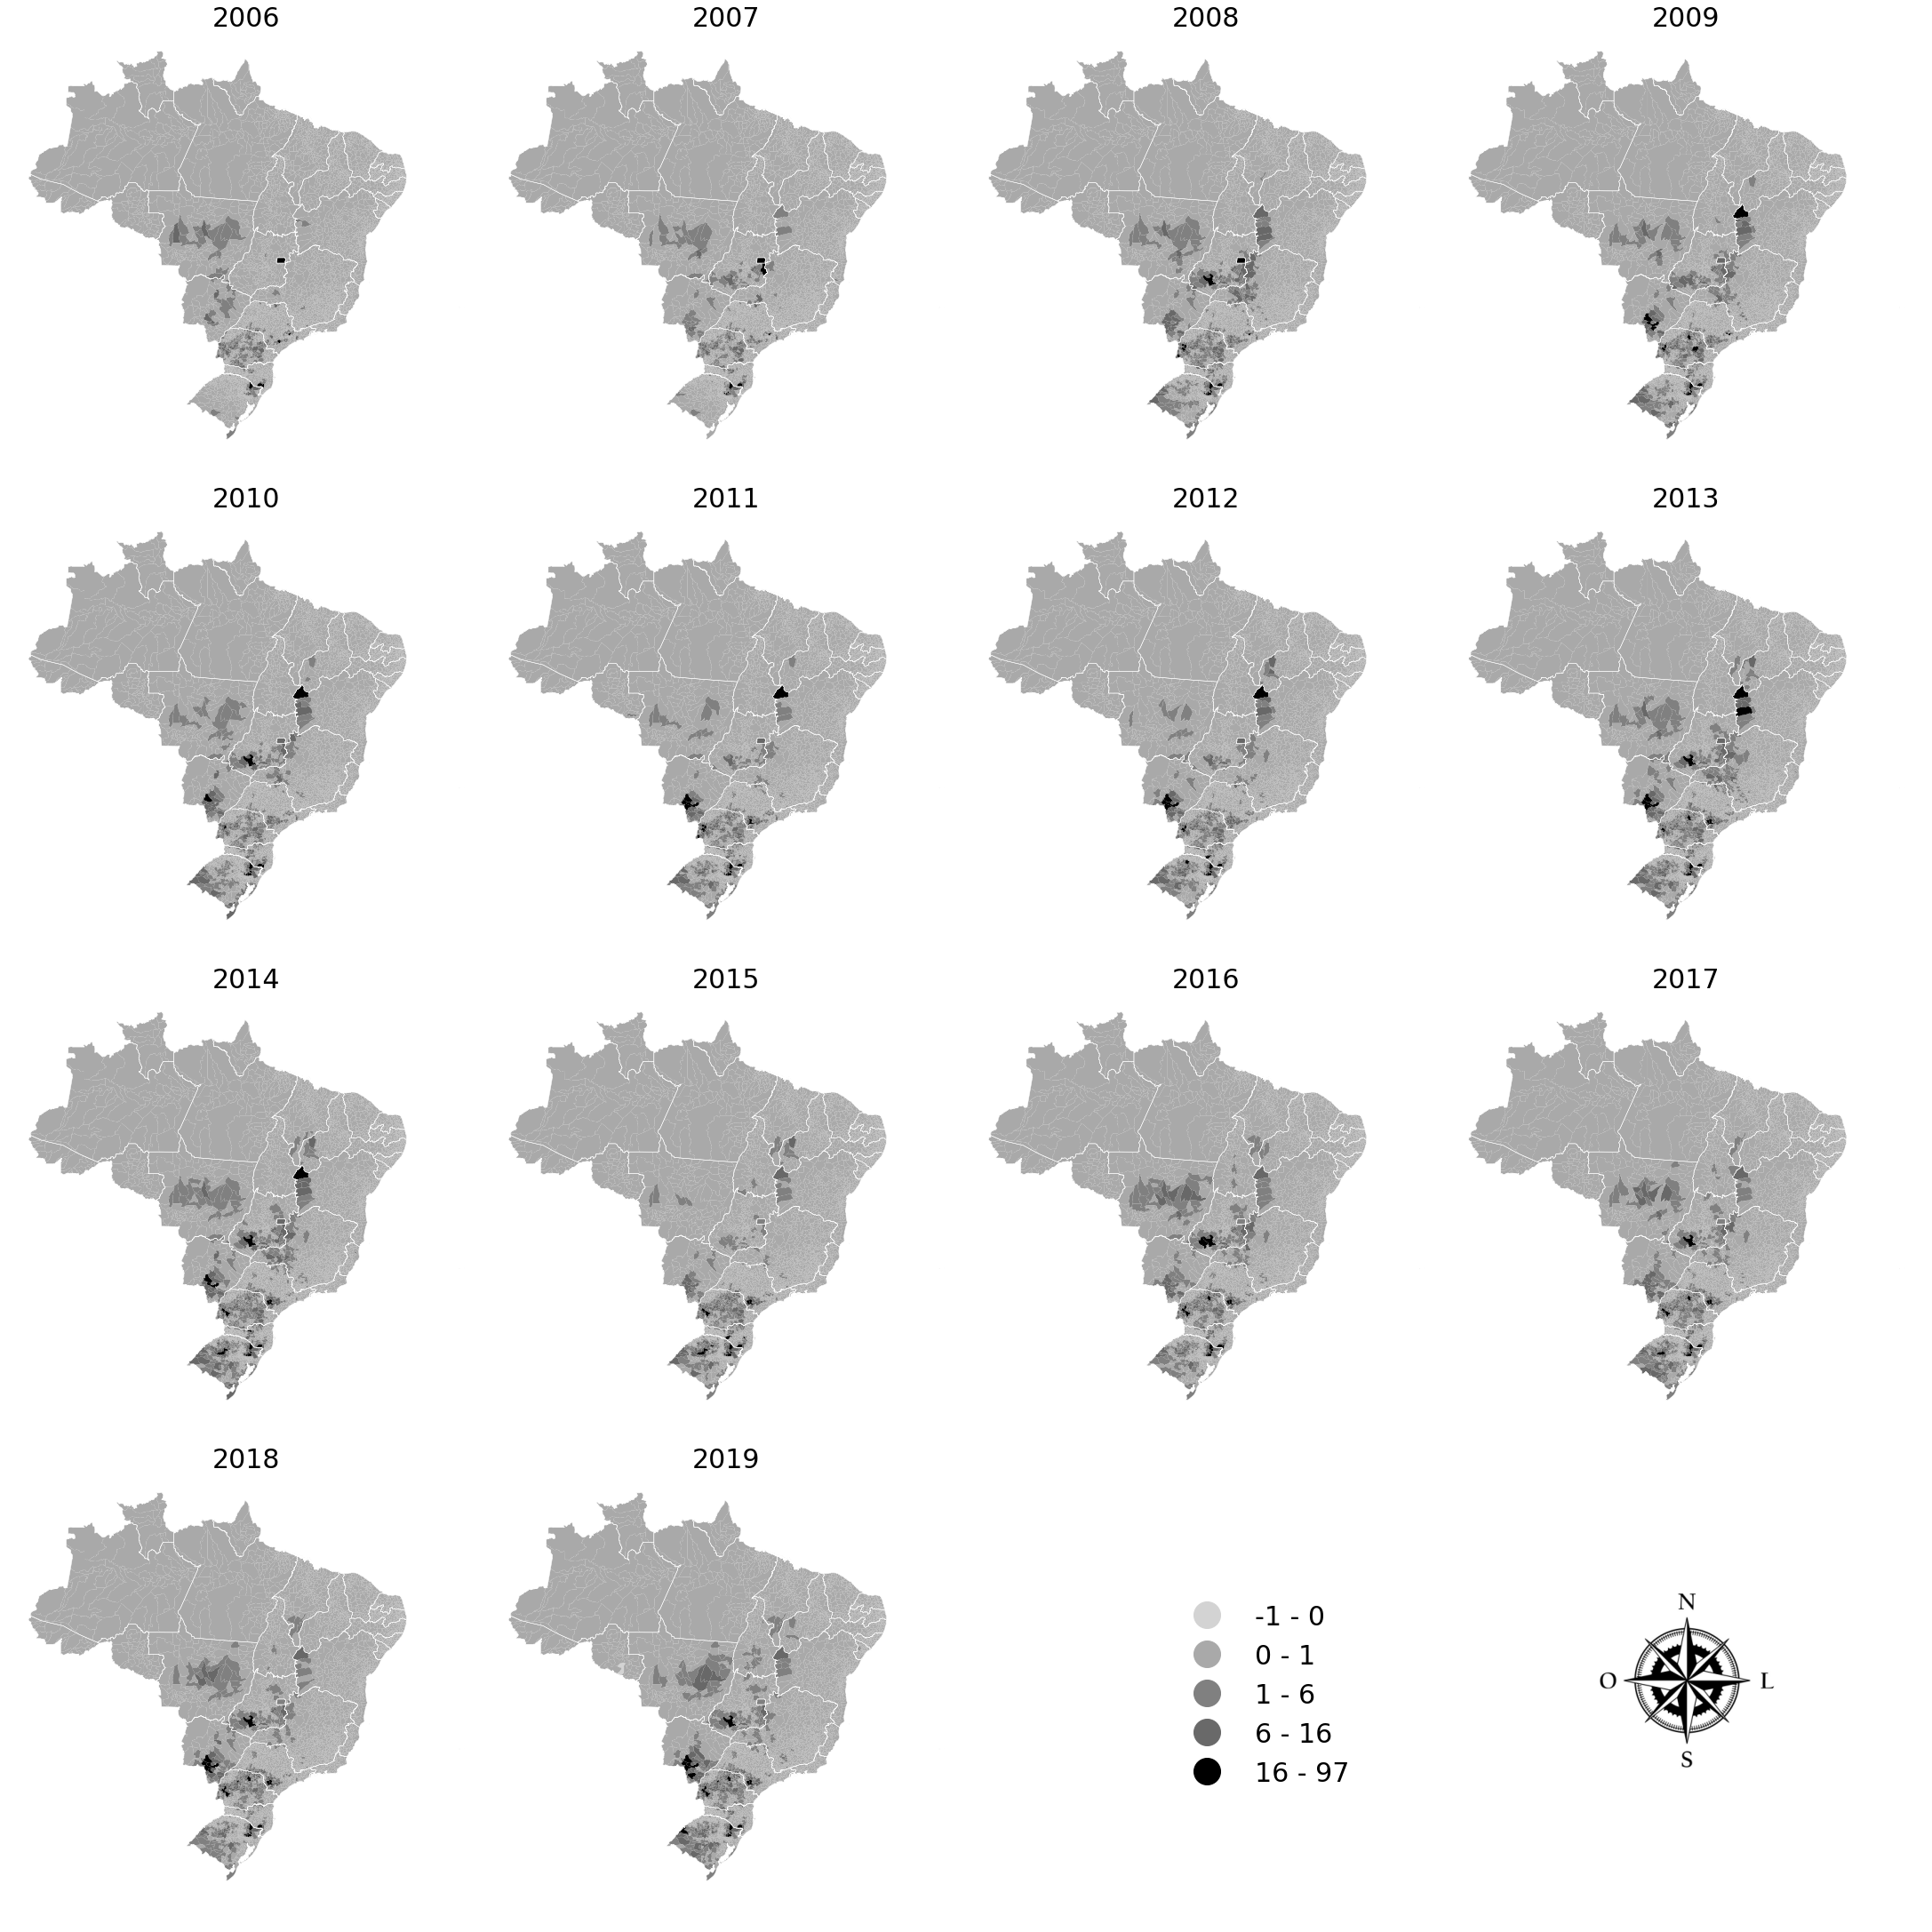
\includegraphics[width=0.9\textwidth]{figuras/map_CP1.png}\\
	\small \textsuperscript {Fonte: Elaboração própria.}
    \label{map_cp1}
\end{figure}

\begin{figure}[H]
	\centering
	\caption{Autocorrelação espacial (\textit{I} de Moran) do primeiro componente principal. Brasil $2006$ -- $2019$}
	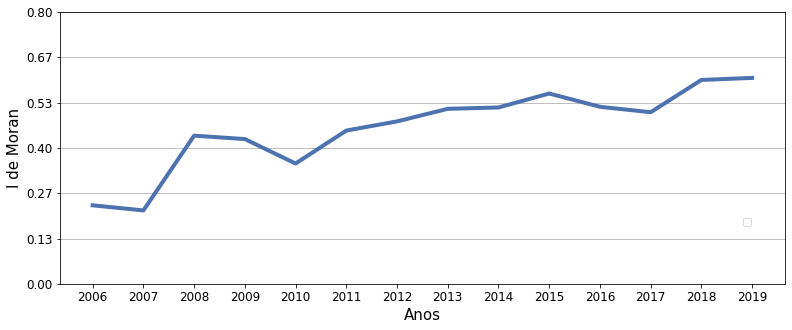
\includegraphics[width=0.8\textwidth]{figuras/i_de_moran_cp1.png}\\
	\small \textsuperscript {Fonte: Elaboração própria.}
    \label{i_moran_cp1}
\end{figure}


\begin{figure}[H]
	\centering
	\caption{Mapas \textit{LISA} para o primeiro componente principal.  Brasil $2006$ -- $2019$.}
	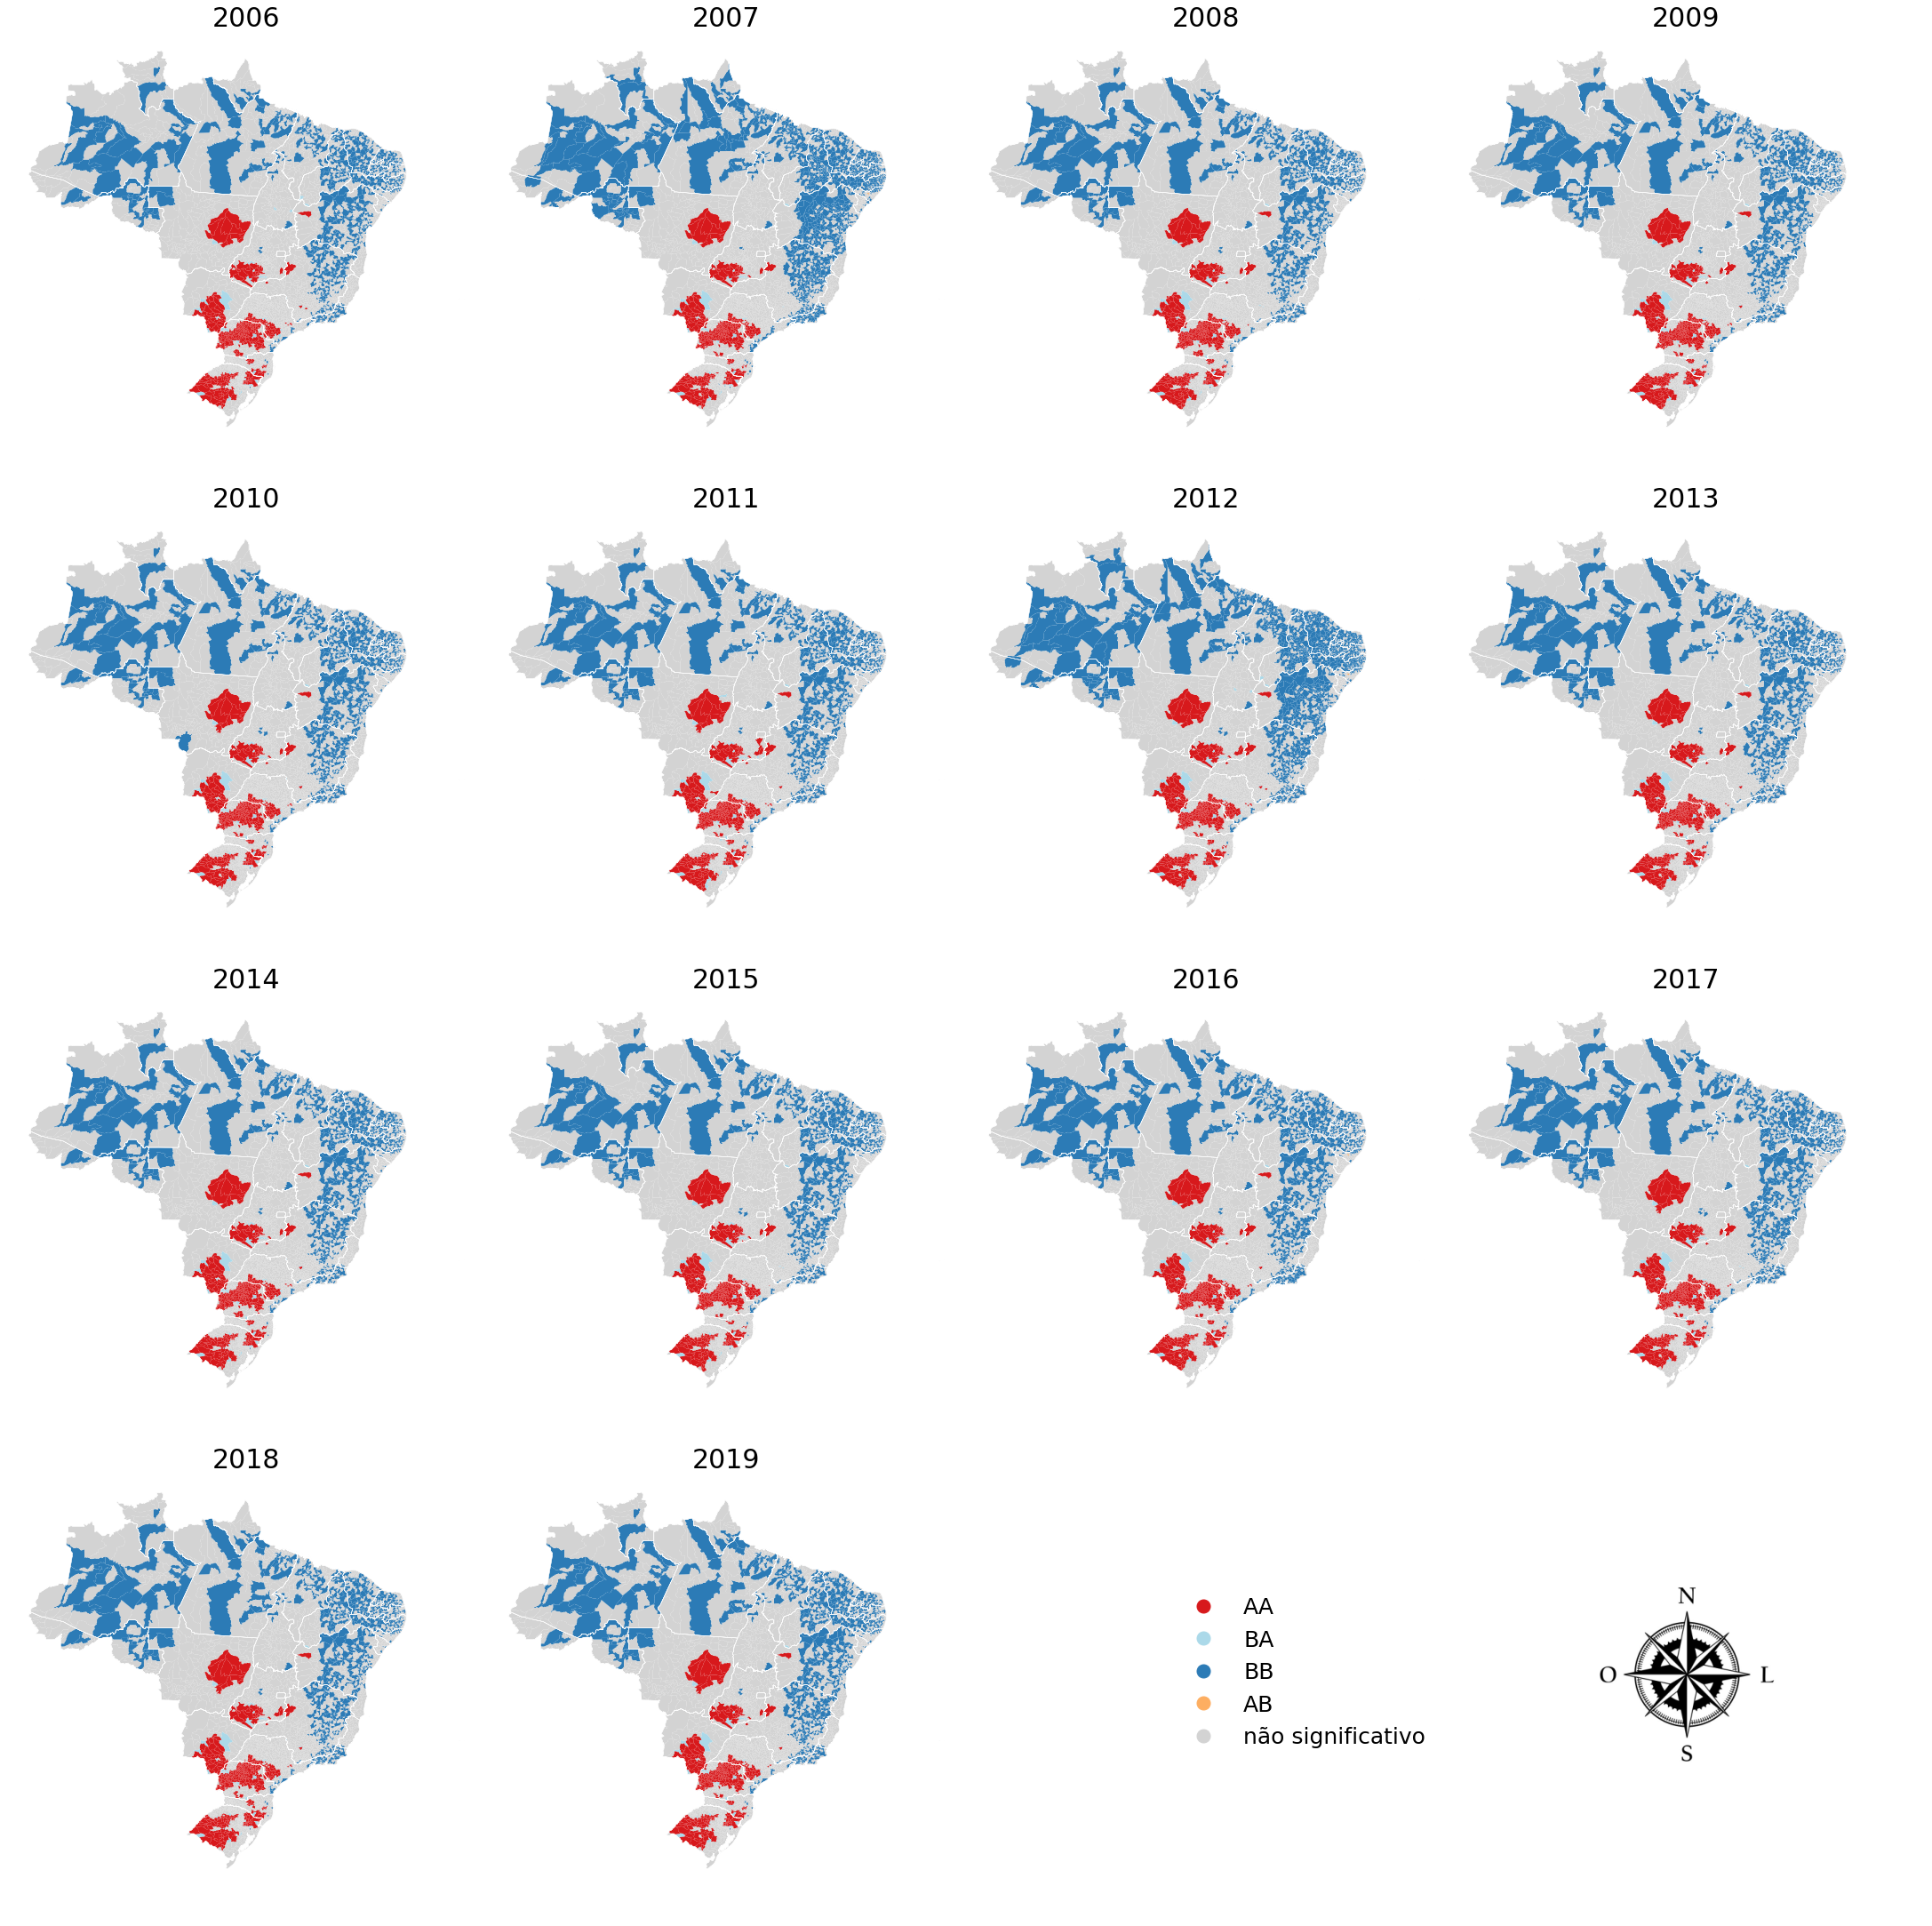
\includegraphics[width=0.9\textwidth]{figuras/map_lisa_cp1.png}\\
	\small \textsuperscript {Fonte: Elaboração própria.}
    \label{map_lisa_cp1}
\end{figure}

\section{CONSIDERAÇÕES FINAIS}\label{sc-conclusion}

\newpage
\addcontentsline{toc}{section}{\hspace*{\distnumber}REFERÊNCIAS}
\begin{center}
\section*{REFERÊNCIAS} 
\end{center}

    
% Use isso descomentado durante edição.
% Quando concluir a Tese, comente iss e use
% o código do bloco abaixo.
%\begin{singlespace}
%\renewcommand\refname{}
%\begin{flushleft}
%\bibliography{../tese/bibtese2}
%\end{flushleft}
%\end{singlespace}

%% Em cap2nlme-corrigido.bbl foi feita correção manual de
%% algumas referências como por exemplo as citações
%% de Dissertação e Tese.
%% Então deixa-se de usar o arquivo cap2nlme.bbl gerado
%% automaticamente pelo abntcite, mas isso é só ao final.
\begin{singlespace}
\begin{flushleft}
\renewcommand\refname{}
\vspace*{-1.5cm}
%==========================================================================================

\documentclass[10pt]{article}

\input{../tese/preambulosimples.tex}

\title{Análise de autocorrelação espacial de dados multivariados de seguro rural}
\date{}

\begin{document}

\maketitle

\begin{abstract}
\input{cap2resumo.tex}
\end{abstract}


\input{cap2.tex}
    
% Use isso descomentado durante edição.
% Quando concluir a Tese, comente iss e use
% o código do bloco abaixo.
%\begin{singlespace}
%\renewcommand\refname{}
%\begin{flushleft}
%\bibliography{../tese/bibtese2}
%\end{flushleft}
%\end{singlespace}

%% Em cap2nlme-corrigido.bbl foi feita correção manual de
%% algumas referências como por exemplo as citações
%% de Dissertação e Tese.
%% Então deixa-se de usar o arquivo cap2nlme.bbl gerado
%% automaticamente pelo abntcite, mas isso é só ao final.
\begin{singlespace}
\begin{flushleft}
\renewcommand\refname{}
\vspace*{-1.5cm}
\input{cap2introduc.bbl}
\end{flushleft}
\end{singlespace}

\newpage
\addcontentsline{toc}{section}{\hspace*{\distnumber}APÊNDICES}
\begin{center}
\section*{APÊNDICES} 
\end{center}

\begin{singlespace}
\noindent{{APÊNDICE A -- } Códigos em Python}
\end{singlespace} 
\vspace{0.25cm}
\begin{small}
\linespread{0.86}
\noindent Código correspondente ao tratamento dos dados. Disponível online em: \url{https://github.com/walefmachado/seguro_rural_espacial/blob/main/scripts/seguro_rural_dados.py}

\vspace{0.25cm}

\noindent Código correspondente aos gráficos, mapas e ACP e AEDE. Disponível online em: \url{https://github.com/walefmachado/seguro_rural_espacial/blob/main/scripts/ seguro_rural_cap2.py}
%\input{scripts/SR_DATA.py} 
%\noindent \rule[4mm]{\textwidth}{0.1ex}
\end{small}


\end{document}

%==========================================================================================

\end{flushleft}
\end{singlespace}

\newpage
\addcontentsline{toc}{section}{\hspace*{\distnumber}APÊNDICES}
\begin{center}
\section*{APÊNDICES} 
\end{center}

\begin{singlespace}
\noindent{{APÊNDICE A -- } Códigos em Python}
\end{singlespace} 
\vspace{0.25cm}
\begin{small}
\linespread{0.86}
\noindent Código correspondente ao tratamento dos dados. Disponível online em: \url{https://github.com/walefmachado/seguro_rural_espacial/blob/main/scripts/seguro_rural_dados.py}

\vspace{0.25cm}

\noindent Código correspondente aos gráficos, mapas e ACP e AEDE. Disponível online em: \url{https://github.com/walefmachado/seguro_rural_espacial/blob/main/scripts/ seguro_rural_cap2.py}
%\input{scripts/SR_DATA.py} 
%\noindent \rule[4mm]{\textwidth}{0.1ex}
\end{small}


\end{document}

%==========================================================================================

\end{flushleft}
\end{singlespace}

\newpage
\addcontentsline{toc}{section}{\hspace*{\distnumber}APÊNDICES}
\begin{center}
\section*{APÊNDICES} 
\end{center}

\begin{singlespace}
\noindent{{APÊNDICE A -- } Códigos em Python}
\end{singlespace} 
\vspace{0.25cm}
\begin{small}
\linespread{0.86}
\noindent Código correspondente ao tratamento dos dados. Disponível online em: \url{https://github.com/walefmachado/seguro_rural_espacial/blob/main/scripts/seguro_rural_dados.py}

\vspace{0.25cm}

\noindent Código correspondente aos gráficos, mapas e ACP e AEDE. Disponível online em: \url{https://github.com/walefmachado/seguro_rural_espacial/blob/main/scripts/ seguro_rural_cap2.py}
%\input{scripts/SR_DATA.py} 
%\noindent \rule[4mm]{\textwidth}{0.1ex}
\end{small}


\end{document}

%==========================================================================================

\end{flushleft}
\end{singlespace}

\newpage
\addcontentsline{toc}{section}{\hspace*{\distnumber}APÊNDICES}
\begin{center}
\section*{APÊNDICES} 
\end{center}

\begin{singlespace}
\noindent{{APÊNDICE A -- } Códigos em Python}
\end{singlespace} 
\vspace{0.25cm}
\begin{small}
\linespread{0.86}
\noindent Código correspondente ao tratamento dos dados. Disponível online em: \url{https://github.com/walefmachado/seguro_rural_espacial/blob/main/scripts/seguro_rural_dados.py}

\vspace{0.25cm}

\noindent Código correspondente aos gráficos, mapas e ACP e AEDE. Disponível online em: \url{https://github.com/walefmachado/seguro_rural_espacial/blob/main/scripts/ seguro_rural_cap2.py}
%\input{scripts/SR_DATA.py} 
%\noindent \rule[4mm]{\textwidth}{0.1ex}
\end{small}


\end{document}

%==========================================================================================
